\documentclass[
	12pt,				% tamanho da fonte
	openright,			% capítulos começam em pág ímpar (insere página vazia caso preciso)
	twoside,			% para impressão em recto e verso. Oposto a oneside
	a4paper,			% tamanho do papel.
	%final,
	% -- opções da classe abntex2 --
	%chapter=TITLE,		% títulos de capítulos convertidos em letras maiúsculas
	%section=TITLE,		% títulos de seções convertidos em letras maiúsculas
	%subsection=TITLE,	% títulos de subseções convertidos em letras maiúsculas
	%subsubsection=TITLE,% títulos de subsubseções convertidos em letras maiúsculas
	% -- opções do pacote babel --
	english,			% idioma adicional para hifenização
    french,             % idioma adicional para hifenização
	spanish,			% idioma adicional para hifenização
	brazil				% o último idioma é o principal do documento
	]{abntex2}

\usepackage{lmodern}
\usepackage[T1]{fontenc}
\usepackage[utf8]{inputenc}
\usepackage{indentfirst}
\usepackage{color}
\usepackage{graphicx}
\usepackage{microtype}

\usepackage[brazilian,hyperpageref]{backref}
\usepackage[alf]{abntex2cite}

\usepackage{float}
\usepackage[obeyFinal,colorinlistoftodos,portuguese]{todonotes}
\usepackage{ifdraft}
\usepackage{pdfpages}
\usepackage{booktabs}
\usepackage{longtable}
\usepackage{styles/vagalivre}

\newcommand\foreign[1]{\emph{#1}}

\renewcommand{\backrefpagesname}{Citado na(s) página(s):~}
\renewcommand{\backref}{}
\renewcommand*{\backrefalt}[4]{
	\ifcase #1 %
		Nenhuma citação no texto.%
	\or
		Citado na página #2.%
	\else
		Citado #1 vezes nas páginas #2.%
	\fi}%

% ---
% Cover and front pages information
% ---
\titulo{\projectName: Planejamento do Projeto}
\autor{Paulo André Haacke}
\local{Porto Alegre}
\data{\today}
\orientador{Cristiano Tonietto Galina}
%\coorientador{Nenhum}
\instituicao{%
  Pontifícia Universidade Católica do Rio Grande do Sul -- PUCRS
  \par
  Faculdade de Informática
  \par
  Especialização em Gerenciamento de Projetos com Ênfase em Tecnologia da Informação}
\tipotrabalho{Trabalho de Conclusão de Curso (Pós-Graduação)}
% O preambulo deve conter o tipo do trabalho, o objetivo, 
% o nome da instituição e a área de concentração 
\preambulo{Solução para Gerenciar Eficientemente a Ocupação de Vagas em Estacionamentos Privados.}
% ---

% ---
% PDF appearence configurations

\definecolor{blue}{RGB}{41,5,195}

% PDF information
\makeatletter
\hypersetup{
     	%pagebackref=true,
		pdftitle={\@title}, 
		pdfauthor={\@author},
    	pdfsubject={\imprimirpreambulo},
	    pdfcreator={LaTeX with abnTeX2},
        pdfkeywords={project management}{gerenciamento de projetos}{tecnologia da informação}{estacionamento privado}{automação}, 
		colorlinks=true,       		% false: boxed links; true: colored links
    	linkcolor=blue,          	% color of internal links
    	citecolor=blue,        		% color of links to bibliography
    	filecolor=magenta,      		% color of file links
		urlcolor=blue,
		bookmarksdepth=4
}
\makeatother
% ---

% --- 
% Line and paragraph space
% --- 

% Paragraph size
\setlength{\parindent}{1.3cm}

% Space between paragraphs
\setlength{\parskip}{0.2cm}  % try also \onelineskip

% ---
% Compile index
% ---
\makeindex
% ---

\begin{document}

% Select document language (according to babel packages)
%\selectlanguage{english}
\selectlanguage{brazil}

% Remove extra space between phrases
\frenchspacing

% ----------------------------------------------------------
% PRETEXTUAL ELEMENTS
% ----------------------------------------------------------
%\pretextual
\listoftodos
\clearpage

% ---
% Cover
% ---
\imprimircapa
% ---

% ---
% Front page
% (The * imply in the existence of a bibliography)
% ---
\imprimirfolhaderosto*
% ---

% ---
% Cataloguing data
% ---

% Isto é um exemplo de Ficha Catalográfica, ou ``Dados internacionais de
% catalogação-na-publicação''. Você pode utilizar este modelo como referência. 
% Porém, provavelmente a biblioteca da sua universidade lhe fornecerá um PDF
% com a ficha catalográfica definitiva após a defesa do trabalho. Quando estiver
% com o documento, salve-o como PDF no diretório do seu projeto e substitua todo
% o conteúdo de implementação deste arquivo pelo comando abaixo:
%
% \begin{fichacatalografica}
%     \includepdf{fig_ficha_catalografica.pdf}
% \end{fichacatalografica}

\begin{fichacatalografica}
	\sffamily
	\vspace*{\fill}					% Posição vertical
	\begin{center}					% Minipage Centralizado
		\fbox{\begin{minipage}[c][8cm]{13.5cm}		% Largura
				\small
				\imprimirautor
				%Sobrenome, Nome do autor

				\hspace{0.5cm} \imprimirtitulo  / \imprimirautor. --
				\imprimirlocal, \imprimirdata-

				\hspace{0.5cm} \pageref{LastPage} p. : il. (algumas color.) ; 30 cm.\\

				\hspace{0.5cm} \imprimirorientadorRotulo~\imprimirorientador\\

				\hspace{0.5cm}
				\parbox[t]{\textwidth}{\imprimirtipotrabalho~--~\imprimirinstituicao,
					\imprimirdata.}\\

				\hspace{0.5cm}
				1. Palavra-chave1.
				2. Palavra-chave2.
				2. Palavra-chave3.
				I. Orientador.
				II. Universidade xxx.
				III. Faculdade de xxx.
				IV. Título
			\end{minipage}}
	\end{center}
\end{fichacatalografica}
% ---

% ---
% Approval page
% ---

% Isto é um exemplo de Folha de aprovação, elemento obrigatório da NBR
% 14724/2011 (seção 4.2.1.3). Você pode utilizar este modelo até a aprovação
% do trabalho. Após isso, substitua todo o conteúdo deste arquivo por uma
% imagem da página assinada pela banca com o comando abaixo:
%
% \includepdf{folhadeaprovacao_final.pdf}
%
\begin{folhadeaprovacao}

	\begin{center}
		{\ABNTEXchapterfont\large\imprimirautor}

		\vspace*{\fill}\vspace*{\fill}
		\begin{center}
			\ABNTEXchapterfont\bfseries\Large\imprimirtitulo
		\end{center}
		\vspace*{\fill}

		\hspace{.45\textwidth}
		\begin{minipage}{.5\textwidth}
			\imprimirpreambulo
		\end{minipage}%
		\vspace*{\fill}
	\end{center}

	Trabalho aprovado. \imprimirlocal, 02 de agosto de 2017:

	\assinatura{\textbf{\imprimirorientador} \\ Orientador}
	\assinatura{\textbf{Professor} \\ Convidado 1}
	\assinatura{\textbf{Professor} \\ Convidado 2}
	%\assinatura{\textbf{Professor} \\ Convidado 3}
	%\assinatura{\textbf{Professor} \\ Convidado 4}

	\begin{center}
		\vspace*{0.5cm}
		{\large\imprimirlocal}
		\par
		{\large\imprimirdata}
		\vspace*{1cm}
	\end{center}

\end{folhadeaprovacao}
% ---

% ---
% Dedication
% ---
\begin{dedicatoria}
	\vspace*{\fill}
	\centering
	\noindent
	\textit{ Este trabalho é dedicado às ...} \vspace*{\fill}
\end{dedicatoria}
% ---

% ---
% Acknowledgment
% ---
\begin{agradecimentos}
	Meus agradecimentos.

\end{agradecimentos}
% ---

% ---
% Epigraph
% ---
\begin{epigrafe}
	\vspace*{\fill}
	\begin{flushright}
		\textit{``Frase inspiradora!''}
		% Sugestoes:
		% - "Não há nada permanente, exceto as mudanças." Heráclito, 500 a.C.
		% - "Lost time is never found again." Benjamin Franklin
		% - "Se eu tivesse oito horas para derrubar uma árvore, passaria seis afiando meu machado." Abraham Lincoln
	\end{flushright}
\end{epigrafe}
% ---

% ---
% ABSTRACTS
% ---

% brazilian portuguese abstract
\setlength{\absparsep}{18pt} % ajusta o espaçamento dos parágrafos do resumo
\begin{resumo}

Ao observar e conversar com donos de estacionamentos privados, assim como com motoristas, percebeu-se dois grandes problemas enfrentados por estes grupos. Os donos e gerentes de estacionamentos privados reportaram a necessidade de aumentar a eficiência e diminuir custos em seus negócios. Os motoristas apontam o tempo gasto com a busca de vagas de garagem e a falta de possibilidade de reservar uma vaga como os principais motivos para a insatisfação com o uso de serviços oferecidos por estacionamentos privados. 

Observando-se estes problemas, percebeu-se que eles complementam um ao outro, e para resolver o problema de um é preciso resolver o problema do outro. Este fato levou à percepção de que a criação de um espécie de leilão de vagas para estacionamentos pode ser uma boa oportunidade de negócio. O plano de projeto para implementação desta idéia é o proposto neste trabalho. 

A solução encontrada aborda a implementação de dois aplicativos. Um para ser utilizado pelo motorista, onde é possível realizar reservas e encontrar estacionamentos vagos. O outro aplicativo foca no dono ou gerente do estacionamento privado, e permite verificar a ocupação do estacionamento, seus horários de pico, controlar entrada e saída de clientes, gerar relatórios de tendências, entre outras funcionalidades.

Este plano de projeto foi baseado nos conhecimentos propostos na quinta edição do \cite{project2013guia}. A organização deste trabalho segue conforme os grupos de processos e as áreas de conhecimento para cada documento criado. O plano foca em apresentar e descrever os processos utilizados durante o gerenciamento deste projeto.

 \textbf{Palavras-chave}: vaga-livre, estacionamento privado, plano de projeto, PMBOK.
\end{resumo}

% english abstract
\begin{resumo}[Abstract]
 \begin{otherlanguage*}{english}
   This is the english abstract.
   \todo[inline,color=green]{Criar abstract.}

   \vspace{\onelineskip}
 
   \noindent 
   \textbf{Keywords}: latex. abntex. text editoration.
 \end{otherlanguage*}
\end{resumo}

% ---
% illustrations list
% ---
\pdfbookmark[0]{\listfigurename}{lof}
\listoffigures*
\cleardoublepage
% ---

% ---
% tables list
% ---
\pdfbookmark[0]{\listtablename}{lot}
\listoftables*
\cleardoublepage
% ---

% ---
% Abbreviations and acronyms list
% ---
\begin{siglas}
	\item[ABNT] Associação Brasileira de Normas Técnicas
\end{siglas}
% ---

% ---
% Symbols list
% ---
%\begin{simbolos}
%	\item[$ \Gamma $] Letra grega Gama
%	\item[$ \Lambda $] Lambda
%	\item[$ \zeta $] Letra grega minúscula zeta
%	\item[$ \in $] Pertence
%\end{simbolos}
% ---

% ---
% Summary
% ---
\pdfbookmark[0]{\contentsname}{toc}
\tableofcontents*
\cleardoublepage
% ---

% ----------------------------------------------------------
% TEXTUAL ELEMENTS
% ----------------------------------------------------------
\textual

% ----------------------------------------------------------
% Introdução (exemplo de capítulo sem numeração, mas presente no Sumário)
% ----------------------------------------------------------
\chapter*[Introdução]{Introdução}
\addcontentsline{toc}{chapter}{Introdução}
% ----------------------------------------------------------

Teste

\chapter{Processos de Iniciação}

% Identificação do GP e sua alçada
% Identificação do Sponsor (nominalmente) 
% Descrição sucinta do projeto e seus objetivos
% Principais stakeholders
% Duração, Data de início e fim
% Orçamento aprovado
% Riscos macro do projeto
% Premissas e restrições

\chapter{Termo de abertura}

\section{Nome do projeto}

\projectName{}.

\section{Patrocinador}

\projectSponsorName{}

%Poderia colocar a minha empresa ou uma empresa contratante, provisoriamente deixei como sendo minha empresa
%Nome e autoridade do patrocinador ou outra(s) pessoa(s) que autoriza(m) o termo de abertura do projeto.

\section{Gerente de projeto}

\projectManagerName{}{} é o gerente de projeto. Sua autoridade é total em relação ao desenvolvimento do produto, podendo contratar, realizar compras e gerenciar o pessoal de acordo com seus próprios critérios.

Em relação ao aspecto financeiro, a autoridade do gerente de projeto estará limitada a determinadas autonomias, a serem definidas no plano de gerenciamento de custos.

%Gerente do projeto, responsabilidade, nível de autoridade designados.

\section{Descrição}

Habilitar gerentes de estacionamentos privados a controlar a ocupação de vagas em seu estacionamento, incluindo visualizar o histórico de ocupação e demanda atual, oferecer um serviço de reserva com rígido controle.

O consumidor será beneficiado através de um aplicativo móvel, onde poderá realizar reservas e encontrar vagas em estacionamentos diversos.

%Descrição de alto nível do projeto e seus limites.

\section{Justificativa}

O mercado de estacionamentos privados tem evoluído muito no Brasil e no Mundo, essa evolução trouxe grandes benefícios para o usuário, entretanto ainda existe demanda para a melhoria nos serviços em áres pouco exploradas, como a busca de vagas e o congestionamento dos estacionamentos e das cidades.

Por outro lado estacionamentos privados encontram dificuldades em alocar de forma eficiente seus estacionamentos.

Neste contexto este projeto pretende apresentar um projeto que possa solucionar os principais problemas encontrados por consumidores e donos de estacionamentos privados.

O desenvolvimento deste sistema pretende trazer as seguintes vantagens para os donos de estacionamentos privados:
\begin{itemize}
	\item Maximizar a ocupação dos estacionamentos.% O que significa isso?
	\item Maximizar o lucro.
	\item Atingir objetivos estratégicos.
	\item Possibilidade de desenvolver estratégias de preço e marketing de acordo com ocupação em períodos anteriores.
	\item Oferecer um melhor serviço aos seus consumidores: permitindo a reserva e busca de vagas.
\end{itemize}

Para os consumidores esta solução pretende trazer os seguintes benefícios:
\begin{itemize}
	\item Diminuir o tempo gasto na busca de vagas para estacionar.
	\item Aumentar a capacidade de busca dos motoristas.
	\item Possibilitar a reserva de vagas.
\end{itemize}

\section{Objetivos}

%%Diminuir o tempo médio de espera em fila para 10 minutos. Diminuir o número de vagas não ocupadas nos piores horários para 50.

\begin{itemize}
	\item Desenvolver um aplicativo de celular portável tanto para Android quanto para IOS para encontrar e reservar vagas de estacionamento.
	\item Desenvolver um software que permita aos estacionamento privados controlar a demanda e ocupação de seus estacionamentos.
	\item O aplicativo e o software devem estar prontos até \maximumDeadline{}.
	\item O aplicativo deve suportar até \minimumUsersAmount{}\ usuários.
\end{itemize}

%Objetivos mensuráveis do projeto e critérios de sucesso relacionados.

%\section{Requisitos}

%Requisitos de alto nível.

\section{Premissas iniciais}

\begin{itemize}
	\item Os estacionamentos privados de Porto Alegre estão prontos para aderir a este tipo de tecnologia.
	\item Disponibilidade do patrocinador: durante o planejamento no mínimo 40\% do tempo, e durante a execução no mínimo 80\% do tempo.
\end{itemize}

\section{Restrições iniciais}

\begin{itemize}
	\item O orçamento é limitado a \maximumBudget{}.
	\item Data máxima para conclusão do projeto: \maximumDeadline{}.
	\item Utilizar base de dados em cloud.
	\item Utilizar um framework multi-plataforma para o desenvolvimento do aplicativo para dispositivos móveis.
\end{itemize}

\section{Riscos iniciais}

\begin{itemize}
	\item Segurança das informações: dados de usuários e transações financeiras.
	\item Atraso nas entregas.
	\item Equipe insuficiente ou indisponível.
	\item Falta de aderência dos estacionamentos privados. %VER
\end{itemize}

\section{Estimativa de Custo}

\maximumBudget{}.

\section{Estimativa de Prazo}

Até \maximumDeadline{}.

\section{Partes interessadas iniciais}

\begin{itemize}
	\item Equipe do projeto.
	\item Patrocinador.
	\item Pessoas (jurídicas e físicas) que utilizam de serviços de estacionamentos privados.
	\item Motoristas que compartilham a estrada com carros em busca de estacionamento.
	\item Funcionários e donos de empreendimentos na área de estacionamentos privados.
	\item Organizações que possuem interesse ou sofrem influência de políticas relacionadas ao meio ambiente.
	\item Fabricantes de automóveis.
	\item Empresas de transporte coletivo.
\end{itemize}

%\section{Requisitos para aprovação do projeto}

%Requisitos para aprovação do projeto (ou seja, o que constitui o sucesso do projeto, quem decide se
%o projeto é bem sucedido e quem assina o projeto).

\section{Controle de Versão}

\begin{table}[H]
	\begin{tabularx}{\textwidth}{| c | c | X | X |}
		\hline
		\textbf{Versão} & \textbf{Data} & \textbf{Autor}        & \textbf{Notas de Revisão}           \\
		\hline
		1                &               & \projectManagerName{} & Criação do documento               \\
		2                &               & \projectManagerName{} & Revisão de premissas e restrições \\
		\hline
	\end{tabularx}
	\centering
\end{table}

\section{Aprovações}

\begin{table}[H]
	\begin{tabularx}{\textwidth}{| c | c | X | c |}
		\hline
		\textbf{Função}  & \textbf{Nome}         & \textbf{Assinatura}        & \textbf{Data} \\
		\hline
		Patrocinador       & \projectSponsorName{} & \projectSponsorSignature{} &               \\
		\hline
		Gerente de projeto & \projectManagerName{} & \projectManagerSignature{} &               \\
		\hline
	\end{tabularx}
	\centering
\end{table}

\section{Identificar Partes Interessadas}

\todo[inline,color=red]{Identificar partes interessadas.}

\chapter{Processos de Planejamento}

%---Escopo
%Descrição do processo utilizado para Gerenciamento do Escopo
%Descrição dos processos de coleta de requisitos
%	Descrição de como os requisitos serão coletados
%	Frequência/ número de eventos de coleta/ limite para cessar a coleta
%	Eventos listados na Matriz de Comunicações
%Descrição do processo de validação e controle do escopo do projeto
%	Descrição de como os requisitos serão validados e controlados
%	Frequência das validações e controle
%	Eventos listados na Matriz de Comunicações
%	Remete ao Controle Integrado de Mudanças em caso de divergência planejado x realizado
%---


\chapter{Plano de gerenciamento de escopo}

\section{Objetivo do documento}

O objetivo deste documento é descrever como será gerenciado o escopo, descrevendo quais ferramentas, técnicas e artefatos serão utilizados para determinar o que deve ser abordado durante o projeto \projectName.

\section{Descrição dos processos de gerenciamento de escopo}

\begin{itemize}
	\item O gerenciamento do escopo do projeto será realizado com base em 3 documentos: declaração de escopo para o escopo funcional do projeto, EAP para o escopo das atividades a serem realizadas pelo projeto e dicionário da EAP para descrever os pacotes de trabalho.
	\item Serão consideradas mudanças de escopo apenas as medidas corretivas. Inovações e novas características do produto ou projeto deverão ser tratados de acordo com o plano de gerenciamento da configuração (ver capítulo \ref{ch:configuration-management-plan}).
	\item Todas as mudanças de escopo deverão ser submetidas por escrito ou através de e-mail, conforme descrito no plano de comunicações do projeto.
\end{itemize}

\section{Priorização das mudanças de escopo e respostas}

\todo[inline,color=orange]{Criar níveis de priorização para as mudanças de escopo ou referenciar modelo de priorização integrado de mudanças.}

\section{Gerenciamento de configuração}

\todo[inline,color=orange]{Referenciar fluxo de controle integrado de mudanças.}

\section{Frequência de avaliação do escopo do projeto}

O escopo deve ser avaliado semanalmente dentro da reunião do CCM, prevista no plano de gerenciamento das comunicações (ver capítulo \ref{ch:communication-management-plan}).

\section{Alocação financeira das mudanças de escopo}

As mudanças de escopo podem ser alocadas dentro das reservas gerenciais do projeto de acordo com as necessidades do gerente de projeto.

Para mudanças de escopo prioritárias, em momentos que não existam mais reservas gerenciais disponíveis, deverá ser acionado o patrocinador, já que o gerente de projeto não possui autonomia para decidir utilizar a reserva de contingência de riscos para mudanças de escopo.

\section{Administração do plano de gerenciamento do escopo}

\subsection{Responsável}

\begin{itemize}
	\item \projectManagerName, gerente de projeto, será o responsável direto pelo plano de gerenciamento de escopo.
\end{itemize}
\todo[inline,color=orange]{Verificar necessidade de adicionar suplente responsável.}

\subsection{Frequência de atualização}

O plano de gerenciamento do escopo será reavaliado mensalmente durante a reunião do CCM, juntamente com os outros planos de gerenciamento do projeto.

\section{Outros assuntos relacionados ao gerenciamento do escopo do projeto não previstos neste plano}

As solicitações não previstas neste plano deverão ser submetidas a reunião do CCM para aprovação.
\todo[inline,color=orange]{Adicionar menção ao plano de mudanças}

\section{Controle de Versão}

\begin{table}[H]
	\begin{tabularx}{\textwidth}{| c | c | X | X |}
		\hline
		\textbf{Versão} & \textbf{Data} & \textbf{Autor}      & \textbf{Notas de Revisão} \\
		\hline
		1                &               & \projectManagerName & Criação do documento     \\
		\hline
	\end{tabularx}
	\centering
\end{table}

\section{Aprovações}

\begin{table}[H]
	\begin{tabularx}{\textwidth}{| c | c | X | c |}
		\hline
		\textbf{Função}  & \textbf{Nome}       & \textbf{Assinatura}      & \textbf{Data} \\
		\hline
		Gerente de projeto & \projectManagerName & \projectManagerSignature &               \\
		\hline
	\end{tabularx}
	\centering
\end{table}

%Tempo
%Descrição do processo de definição das atividades (base na decomposição dos pacotes da EAP normalmente)
%Descrição do processo e técnicas de sequenciamento das atividades
%Descrição do processo de estimativa de recursos para as atividades
%Descrição do método de gerenciamento do tempo que será empregado no projeto (PERT/CPM, corrente crítica, SCRUM, ...) e a justificativa para sua aplicação no projeto
%Elementos visuais:
%   Visão executiva do cronograma em formato gráfico (Gantt, Burndown, ...), deve ocupar apenas uma página
%   Principais marcos do projeto na visão do cliente final, patrocinador ou gerência imediata / tem no escopo
%   Cronograma detalhado do projeto com identificação do caminho crítico no formato Gantt contendo: Atividade, Duração, Data de início, Data de fim, Percentual de progresso
%   Lista de atividades do caminho crítico com datas de início e fim
%Apresentação do processo empregado para gerenciamento da linha de base de tempo
%Descrição do processo de controle do cronograma
%   Frequência das ações de controle
%   Eventos listados na Matriz de Comunicações
%   Remete ao Controle Integrado de Mudanças em caso de divergência planejado x realizado

\chapter{Plano de gerenciamento do cronograma}

\section{Descrição dos processos de gerenciamento de tempo}

\begin{itemize}
	\item O gerenciamento de cronograma será realizado a partir da alocação de precentual completo nas atividades do projeto através da utilização do software \projectManagementSoftwareName.
    \item Utilizando o método da corrente crítica o gerente de projeto criou o cronograma do projeto. O gráfico de Gannt representando o cronograma encontra-se no apêndice \ref{ch:gannt-chart}.
	\item A atualização dos prazos do projeto será realizada no sofwtare \projectManagementSoftwareName através da publicação no repositório de documentos do projeto dos seguintes relatórios:
	      \begin{itemize}
		      \item Gráfico de Gannt;
		      \item Diagrama de rede;
		      \item Percentual completo.
	      \end{itemize}
	\item A avaliação de desempenho do projeto será realizada através da análise de valor agregado, onde o custo e o prazo do projeto são acompanhados em um único processo de controle.
	\item Todas atividades com folga menor ou igual a 3 dias serão consideradas críticas.
	\item Todas mudanças no prazo inicialmente previsto para o projeto devem ser avaliadas e classificadas de acordo com o sistema de controle integrado de mudanças (ver seção \ref{sec:change-control-system}).
	\item Atrasos decorrentes de medidas corretivas e que influenciam no sucesso do projeto serão integrados ao plano. Novos recursos terão seus prazos negociados na reunião do CCM.
	\item Atualizações na linha de base do projeto somente serão permitidas com autorização expressa do gerente de projeto e do patrocinador. A linha de base anterior deve ser arquivada, documentada e publicada para fins de lições aprendidas.
	\item Solicitações de mudanças no crognorama definido deverão ser realizadas através do formulário de requisição de mudança (ver apêndice \ref{ch:change-request-form}), conforme previsto no plano de gerenciamento das mudanças (ver capítulo \ref{ch:change-management-plan})
\end{itemize}

\section{Priorização das mudanças nos prazos e respostas}

As mudanças nos prazos deverão ser classificadas de acordo com o modelo de priorização integrada de mudanças (ver seção \ref{sec:integrated-change-priorization}).

\section{Sistema de controle de mudanças de prazos}

Todas as mudanças nos prazos e atrasos/adiantamentos do projeto devem ser tratados segundo o fluxo apresentado pelo sistema de controle integrado das mudanças (ver seção \ref{sec:change-control-system}).

%\section{Mecanismo adotado para conflitos de recursos}

\section{Buffer de tempo do projeto}

O projeto adotará o conceito de corrente crítica, tendo cada atividade seu \emph{pulmão}. Deverão ser criados pulmões de caminho para proteger uma corrente crítica e também pulmões de projeto, para proteger a data final do projeto contra possíveis problemas.

Para gerenciar estes pulmões o gerente de projeto deverá dividir cada pulmão em três partes. Enquanto o uso estiver no primeiro terço se considera que está controlado. No segundo terço o gerente de projeto volta sua atenção para as atividades relacionadas a este pulmão e busca descobrir se existem indícios de que a atividade não irá terminar no prazo, se encontrar tais indícios o gerente de projeto pode trazer os mesmos para serem discutidos durante a reunião semanal do CCM. Se já estiver utilizando o último terço do pulmão o gerente de projeto deve acionar o CCM solicitando uma mudança de prazo ou escopo.

\section{Frequência de avaliação dos prazos do projeto}

Os prazos do projeto deverão ser avaliados e atualizados semanalmente, sendo os resultados publicados no repositório de documentos do projeto e apresentados durante a reunião semanal do CCM, pervista no plano de gerenciamento das comunicações.

\section{Alocação financeira para o gerenciamento de tempo}

As mudanças de recuperação de atraso no projeto que requerem gastos adicionais podem ser alocadas dentro das reservas gerenciais do projeto de acordo com as necessidades do gerente de projeto.

Em caso que haja necesidade de medidas prioritárias para a recuperação de prazos, em momentos que não existam mais reservas gerenciais disponíveis, deverá ser acionado o patrocinador, já que o gerente de projeto não possui autonomia para decidir utilizar a reserva de contingência de riscos para a recuperação de atrasos.

\section{Administração do plano de gerenciamento de tempo}

\subsection{Responsável}

\begin{itemize}
	\item \projectManagerName, gerente de projeto, será o responsável direto pelo plano de gerenciamento do cronograma.
\end{itemize}

\subsection{Frequência de atualização}

O plano de gerenciamento do cronograma será reavaliado mensalmente durante a reunião do CCM, juntamente com os outros planos de gerenciamento do projeto.

\section{Outros assuntos relacionados ao gerenciamento do cronograma do projeto não previstos neste plano}

Solicitações não previstas neste plano deverão ser submetidas a reunião do CCM para aprovação. O plano de gerenciamento do cronograma deverá ser atualizado com as devidas alterações realizadas.

\section{Controle de Versão}

\begin{table}[H]
	\begin{tabularx}{\textwidth}{| c | c | X | X |}
		\hline
		\textbf{Versão} & \textbf{Data} & \textbf{Autor}      & \textbf{Notas de Revisão} \\
		\hline
		1                &               & \projectManagerName & Criação do documento     \\
		\hline
	\end{tabularx}
	\centering
\end{table}

\section{Aprovações}

\begin{table}[H]
	\begin{tabularx}{\textwidth}{| c | c | X | c |}
		\hline
		\textbf{Função}  & \textbf{Nome}       & \textbf{Assinatura}      & \textbf{Data} \\
		\hline
		Patrocinador       & \projectSponsorName & \projectSponsorSignature &               \\
		\hline
		Gerente de projeto & \projectManagerName & \projectManagerSignature &               \\
		\hline
	\end{tabularx}
	\centering
\end{table}

% Descrição do método de gerenciamento do custo a ser empregado no projeto incluindo: Sistema de alocação de custos, Relatórios de controle, Periodicidade de atualização
% Método de estimativa dos custos
% Apresentação da composição de valores que totalizam o custo do projeto incluindo: 
%   Custo com pessoal
%   Aquisições
%   Reservas Gerenciais
%   Reservas de Contingência (oriunda dos riscos)
%   Outros
% EVA – Análise de Valor Agregado do Projeto (simulação em momento projetado):
%   Aplicação do método de EVA no projeto
%   Detalhamento dos índices utilizados e análise dos resultados
%   Curvas de desempenho
%   Apresentação de análise comparativa entre o orçamento inicial aprovado do projeto e o custo orçado inicialmente para o projeto: Justificar em caso de diferença 
% Modelo de análise e controle de custos do projeto:
%   Comparação do realizado x linha de base de custos do projeto
%   Ações caso existam diferenças
%   Fluxo de caixa
%   Custo final projetado considerando-se o desempenho atual do projeto
% Apresentação dos custos correntes ou potenciais que não serão apropriados ao projeto
% Descrição do processo de controle dos custos
%   Frequência das ações de controle
%   Eventos listados na Matriz de Comunicações
%   Remete ao Controle Integrado de Mudanças em caso de divergência planejado x realizado

\chapter{Plano de gerenciamento dos custos}
\label{ch:cost-management-plan}

%\todo[inline,color=red]{Revisar plano de gerenciamento dos custos.}

%\section{Visão geral}

%O plano de gerenciamento dos custos descreve como os custos do projeto serão planejados, estruturados e controlados fornecendo detalhes sobre os processos e ferramentas utilizados para gerenciar questões relacionadas a custos.

%Os processos e ferramentas descritos neste plano orientam o gerenciamento das atividades vistas na figura \ref{fig:cost-management-plan-flowchart}.

%\begin{figure}[h]
%	\centering
%	\begin{tikzpicture}[node distance = 0.7cm and 0.7cm, auto]
%		\node (estimate) [process] {Estimar Custos};
%		\node (determine-budget) [process, right= of estimate] {Determinar Orçamento};
%		\node (control-costs) [process, right= of determine-budget] {Controlar Custos};
%		\path [line] (estimate) -- (determine-budget);
%		\path [line] (determine-budget) -- (control-costs);
%	\end{tikzpicture}
%	\caption{Processo para gerenciamento dos custos do projeto.}
%	\label{fig:cost-management-plan-flowchart}
%\end{figure}

\section{Descrição dos processos de gerenciamento de custos}

\begin{itemize}
	% Estimar custos
	% Ver custo da qualidade (PMBOK 8.1.2.2)
	\item Utilizando-se o método \foreign{bottom-up} devem ser estimados os custos para cada uma das atividades presentes na EAP.
	\item A estimativativa de custos será conduzida pelo gerente de projetos e apoiada pela opinião especializada da equipe técnica.
	\item Custos que possuam incertezas e riscos significantes deverão utilizar a análise de PERT, conforme equação \ref{eq:cost-pert}.
	      \begin{equation}\label{eq:cost-pert}
		      CE = \frac{CO+4CMP+CP}{6}
	      \end{equation}
	      \begin{description}
		      \item[Custo Estimado (DE):] a melhor estimativa do custo necessário para completar a atividade, levando em consideração o fato de que o projeto nem sempre corre conforme o planejado.
		      \item[Custo Mais Provável (MP):] custo da atividade baseado em um esforço de avaliação realista para o trabalho necessário e quaisquer outros gastos previstos.
		      \item[Custo Otimista (O):] custo da atividade baseado na análise do melhor cenário possível para a atividade.
		      \item[Custo Pessimista (P):] custo da atividade baseado na análise do pior cenário para a atividade.
	      \end{description}
	\item A atualização e gerenciamento dos custos do projeto será realizada utilizando o software \projectManagementSoftwareName{}.
	      % Determinar o orçamento
	\item Custos indiretos não serão considerados nos custos deste projeto.
	      % Controlar custos
	\item A avaliação dos custos será feito por meio da comparação entre 3 estimativas: valor planejado, valor real e valor agregado.
	\item O controle dos custos será feito tomando como base a estimativa de valor agregado (ver apêndice \ref{project-monitoring-report}).
	\item Custos recorrentes de tempo e material, como a contratação de um servidor em nuvem, serão considerados de forma proporcional no período de sua contratação até o encerramento do projeto. Mais detalhes podem ser encontrados no plano de gerenciamento das aquisições, localizado no apêndice \ref{ch:procurement-management-plan}.
\end{itemize}

\section{Frequência de avaliação do orçamento do projeto e das reservas gerenciais}

O orçamento, assim como o uso de reservas gerenciais, do projeto será avaliado semanalmente pelo gerente do projeto.

\section{Orçamento do projeto}

O orçamento do projeto é de \realBudget{}, o que abrange os gastos internos com recursos, aquisições e reservas gerenciais.

\section{Taxa padrão dos recursos}

\begin{longtable}{ p{0.2\textwidth} p{0.2\textwidth} l l l }
	\toprule
	\textbf{Recurso}      & \textbf{Cargo}              & \textbf{Experência} & \textbf{Tipo} & \textbf{Taxa Padrão} \\
	\midrule
	\endhead
	\multicolumn{5}{c}{{\textit{Continua na próxima página.}}} \\
	\caption{Taxa padrão dos recursos.}
	\endfoot
	\endlastfoot
	\ceoName{}            & CEO                         & N/A                  & Trabalho      & R\$ 0,00/hr           \\
	\midrule
	\projectManagerName{} & Gerente do projeto          & Pleno                & Trabalho      & R\$ 67,00/hr          \\
	\midrule
	\mobDevOneName{}      & Desenvolvedor mobile        & Pleno                & Trabalho      & R\$ 50,00/hr          \\
	\midrule
	\mobDevTwoName{}      & Desenvolvedor mobile        & Pleno                & Trabalho      & R\$ 50,00/hr          \\
	\midrule
	\frontWebDevName{}    & Desenvolvedor web front-end & Pleno                & Trabalho      & R\$ 44,00/hr          \\
	\midrule
	\backWebDevName{}     & Desenvolvedor web back-end  & Pleno                & Trabalho      & R\$ 51,00/hr          \\
	\midrule
	\softEngName{}        & Engenheiro de software      & Sênior              & Trabalho      & R\$ 67,00/hr          \\
	\midrule
	\softArcName{}        & Arquiteto de software       & Pleno                & Trabalho      & R\$ 52,00/hr          \\
	\midrule
	\testAnalOneName{}    & Analista de testes          & Sênior              & Trabalho      & R\$ 45,00/hr          \\
	\midrule
	\testAnalTwoName{}    & Analista de testes          & Pleno                & Trabalho      & R\$ 45,00/hr          \\
	\midrule
	\dbAnalName{}         & Analista de banco de dados  & Sênior              & Trabalho      & R\$ 66,00/hr          \\
	\bottomrule
	\caption{Taxa padrão dos recursos.}
	\centering
\end{longtable}

\section{Custos dos recursos do projeto por atividade}

O documento descrevendo o custo de cada atividade no projeto encontra-se no apêndice \ref{ch:activities-cost}.

\section{Aquisições}

Conforme descrito no plano de gerenciamento das aquisições o projeto, estima-se que o projeto terá um gasto de \procurementBudget{} para a contratação do servidor em nuvem durante o período do projeto. Este valor estará incluso no orçamento do projeto.

\section{Reservas gerenciais}

Além da linha de base de custos, o gerente do projeto contará com uma reserva gerencial de 10\% sobre o valor da linha de base, a qual estará diponível em casos de riscos desconhecidos e atividades não identificadas no escopo.

\section{Autonomias}

O gerente do projeto possui autonomia total para uso da reserva contingencial.

O gerente do projeto possui autonomia sobre o uso da reserva gerencial em diferentes eventos. Para cada evento em que haja necessidade de utilizar a reserva gerencial o gerente do projeto possui autonomia conforme descrito na tabela \ref{tab:project-manager-cost-autonomy}.

\begin{table}[h]
	\centering
	\begin{tabular}{| l | l |}
		\hline
		\textbf{Uso da Reserva Gerencial} & \textbf{Autonomia}                                   \\
		\hline
		Até R\$ 3.000,00                 & Gerente do projeto                                   \\
		\hline
		Até R\$ 7.000,00                 & Gerente do projeto com autorização do patrocinador \\
		\hline
		Acima de R\$ 7.000,00             & Apenas o patrocinador                                \\
		\hline
	\end{tabular}
	\caption{Autonomias do gerente de projetos sobre a reserva gerencial.}
	\label{tab:project-manager-cost-autonomy}
\end{table}

A reserva gerencial pode ser utilizada de forma cumulativa. Quando for atingido o limite de 50\% de uso da reserva gerencial o gerente do projeto deve informar o patrocinador.

Para medidas prioritárias ou urgentes que estejam fora da alçada do gerente do projeto, ou na ausência de reserva gerencial disponível o patrocinador deverá ser acionado para a tomada da decisão.

\section{Alocação financeira das mudanças no orçamento}

Conforme descrito no plano de gerenciamento das mudanças (ver capítulo ch:change-management-plan), a reserva gerencial pode ser utilizada caso o gerente do projeto necessite realizar mudanças de orçamento de prioridade média.

Todas as mudanças no orçamento do projeto deverão ser classificadas de acordo com o modelo de priorização integrada de mudanças (ver seção \ref{sec:integrated-change-priorization}), além disso devem seguir conforme o fluxo apresentado pelo sistema de controle integrado das mudanças (ver seção \ref{sec:change-control-system}).

\section{Administração do plano de gerenciamento de custos}

\subsection{Responsável pelo plano}

\begin{itemize}
	\item \projectManagerName{}, gerente de projeto, será o responsável direto pelo plano de gerenciamento do tempo.
\end{itemize}

\subsection{Frequência de atualização do plano de gerenciamento de custos}

O plano de gerenciamento dos custos será reavaliado semanalmente durante a reunião do CCM, juntamente com os outros planos de gerenciamento do projeto.

\section{Outros assuntos relacionados ao gerenciamento de custos do projeto não previstos neste plano}

Solicitações não previstas neste plano deverão passar pela aprovação do CCM. Após aprovada o plano deve ser atualizado pelo gerente do projeto.

\section{Controle de versão}

\begin{table}[H]
	\begin{tabularx}{\textwidth}{| c | c | X | X |}
		\hline
		\textbf{Versão} & \textbf{Data} & \textbf{Autor}        & \textbf{Notas de Revisão}           \\
		\hline
		1                & 23/04/2017    & \projectManagerName{} & Criação do documento               \\
		\hline
		2                & 29/04/2017    & \projectManagerName{} & Corrigindo taxa padrão dos recursos \\
		\hline
		3                & 04/05/2017    & \projectManagerName{} & Adicionando autonomias               \\
		\hline
		4                & 05/05/2017    & \projectManagerName{} & Revisão do documento                \\
		\hline
	\end{tabularx}
	\centering
\end{table}

\section{Aprovações}

\begin{table}[H]
	\begin{tabularx}{\textwidth}{| c | c | X | c |}
		\hline
		\textbf{Função}  & \textbf{Nome}         & \textbf{Assinatura}        & \textbf{Data} \\
		\hline
		Patrocinador       & \projectSponsorName{} & \projectSponsorSignature{} & 06/06/2017    \\
		\hline
		Gerente de projeto & \projectManagerName{} & \projectManagerSignature{} & 06/06/2017    \\
		\hline
	\end{tabularx}
	\centering
\end{table}



%Descrição do processo de garantia da qualidade do projeto e do produto desenvolvido incluindo:
%   Padrões de referência a serem utilizados/ check lists
%   Processos
%   Auditorias
%   Ações em caso de Não Conformidade
%   Ferramentas da qualidade
%Identificação dos indicadores de qualidade do projeto 
%Descrição do processo de verificação da qualidade do projeto
%   Métodos de verificação
%   Frequência das ações de controle
%   Eventos listados na Matriz de Comunicações
%   Remete ao Controle Integrado de Mudanças em caso de divergência planejado x realizado
%   Plano de ações corretivas e preventivas
%Descrição do processo de verificação da qualidade do produto
%   Métodos de verificação
%   Frequência das ações de controle
%   Eventos listados na Matriz de Comunicações
%   Remete ao Controle Integrado de Mudanças em caso de divergência planejado x realizado 
%   Plano de ações corretivas e preventivas

\chapter{Plano de gerenciamento da qualidade}

\section{Responsabilidades na garantia da qualidade}

\todo[inline,color=red]{Terminar definição dos responsáveis pela garantia da qualidade.}

\begin{table}[H]
	\begin{tabularx}{\textwidth}{| c | X |}
		\hline
		\textbf{Papel}     & \textbf{Responsabilidade}                            \\
		\hline
		Gerente de projeto & Especificar o cronograma do projeto incluindo testes \\
		\hline
	\end{tabularx}
	\centering
	\caption{Tabela de responsabilidades na garantia da qualidade.}
\end{table}

\section{Responsabilidades no controle da qualidade}

\todo[inline,color=red]{Terminar definição dos responsáveis pelo controle da qualidade.}

\begin{table}[H]
	\begin{tabularx}{\textwidth}{| c | X |}
		\hline
		\textbf{Papel}     & \textbf{Responsabilidade}                            \\
		\hline
		Gerente de projeto & Especificar o cronograma do projeto incluindo testes \\
		\hline
	\end{tabularx}
	\centering
	\caption{Tabela de responsabilidades no controle da qualidade.}
\end{table}

\section{Processo de gerenciamento da qualidade}

\todo[inline,color=red]{Criar processo para gerenciamento da qualidade.}

\section{Política de gerenciamento da qualidade}

\begin{itemize}
	\item O sistema de controle de mudanças da qualidade deve ser utilizado para verificar e classificar alterações nos requisitos de qualidade.
	\item Mudanças corretivas que impactem no sucesso do proejto serão incorporadas ao plano.
	\item Todas as solicitações de mudanças devem ser realizadas de acordo com o plano de gerenciamento das mudanças (ver capítulo \ref{ch:change-management-plan}).
\end{itemize}

\section{Planejamento de avaliação de qualidade}

O planejamento de avaliação de qualidade seguirá conforme a tabela \ref{tab:quality-evaluation-plan}.

\begin{table}[h]
	\begin{tabularx}{.9\textwidth}{| c | X | X |}
		\hline
		\textbf{Data} & \textbf{Tipo de Avaliação a ser Realizada} & \textbf{Atividades ou Artefatos a serem Revisados} \\
		\hline
		01/08/2017    & Teste Unitário                              & Aplicativo do Motorista                            \\
		\hline
		14/08/2017    & Teste Unitário                              & Aplicativo do Estacionamento                       \\
		\hline
		21/08/2017    & Teste Unitário                              & Software de Centralização                        \\
		\hline
		01/09/2017    & Teste de Integração                        & Aplicativo do Motorista                            \\
		\hline
		30/08/2017    & Teste de Integração                        & Aplicativo do Estacionamento                       \\
		\hline
		03/10/2017    & Teste de Integração                        & Software de Centralização                        \\
		\hline
	\end{tabularx}
	\centering
	\caption{Planejamento de avaliação de qualidade.}
	\label{tab:quality-evaluation-plan}
\end{table}

\section{Planejamento de testes/inspeções}

\subsection{Configuração do ambiente de teste}

\begin{description}
	\item[Plataforma em Nuvem] \hfill
	\begin{itemize}
		\item Plataforma em nuvem com suporte ao SGBD MySQL.
		\item Plataforma em nuvem para disponibilizar aplicativos web.
	\end{itemize}
\end{description}

\begin{description}
	\item[Dispositivo Móvel] \hfill
	\begin{itemize}
		\item Android v4.0 ou superior.
	\end{itemize}
\end{description}

\subsection{Pré-requisitos}

\begin{itemize}
	\item Conhecimento de abordagens e técnicas de teste.
	\item Conhecimento da aplicação e de seu estado.
	\item Conhecimento de negócio e método de utilização do sistema.
	\item Capacidade de resolução de problemas.
\end{itemize}

\section{Frequência de atualização do plano de gerenciamento da qualidade}

Os requisitos de qualidade do projeto devem ser avaliados semanalmente durante a reunião do CCM, prevista no plano de gerenciamento das comunicações.

\section{Alocação financeira das mudanças nos requisitos de qualidade}

As mudanças nos requisitos de qualidade podem ser alocadas dentro das reservas gerenciais do projeto.

Em caso de mudanças prioritárias nos requisitos de qualidade do projeto, quando não existem reservas gerenciais disponíveis, deverá ser acionado o patrocinador.

\section{Priorização das mudanças nos requisitos de qualidade e respostas}

As mudanças nos requisitos de qualidade deverão ser classificadas de acordo com o modelo de priorização integrada de mudanças (ver seção \ref{sec:integrated-change-priorization}).

\section{Sistema de controle de mudanças da qualidade}

Todas as mudanças nos requisitos de qualidade do projeto devem ser tratados segundo o fluxo apresentado pelo sistema de controle integrado das mudanças (ver seção \ref{sec:change-control-system}).

\section{Métricas de qualidade}

As métricas de qualidade encontram-se no apêndice \ref{quality-metrics}.

\section{Administração do plano de gerenciamento da qualidade}

\subsection{Responsável}

\begin{itemize}
	\item \projectManagerName, gerente de projeto, será o responsável direto pelo plano de gerenciamento da qualidade.
\end{itemize}

\section{Outros assuntos relacionados ao gerenciamento da qualidade do projeto não previstos neste plano}

Solicitações não previstas neste plano deverão passar pela aprovação do CCM. Após aprovada o plano deve ser atualizado pelo gerente do projeto.

\section{Controle de Versão}

\begin{table}[H]
	\begin{tabularx}{\textwidth}{| c | c | X | X |}
		\hline
		\textbf{Versão} & \textbf{Data} & \textbf{Autor}      & \textbf{Notas de Revisão} \\
		\hline
		1                &               & \projectManagerName & Criação do documento     \\
		\hline
	\end{tabularx}
	\centering
\end{table}

\section{Aprovações}

\begin{table}[H]
	\begin{tabularx}{\textwidth}{| c | c | X | c |}
		\hline
		\textbf{Função}  & \textbf{Nome}       & \textbf{Assinatura}      & \textbf{Data} \\
		\hline
		Patrocinador       & \projectSponsorName & \projectSponsorSignature &               \\
		\hline
		Gerente de projeto & \projectManagerName & \projectManagerSignature &               \\
		\hline
	\end{tabularx}
	\centering
\end{table}

% Descrição do tipo de estrutura organizacional da empresa onde o projeto está inserido: Projetizada, matricial forte, funcional, Identificar prós e contras do modelo vigente
% Descrição das necessidades de recursos humanos do projeto: Papéis, Competências, Responsabilidades, Quantidades, Relações hierárquicas
% Organograma do projeto (ideal é ter nome + papel)
% Matriz RACI
% Descrição do plano de mobilização da equipe do projeto: Processo de alocação ou contratação, Datas de alocação e saída do projeto
% Descrição do plano de desenvolvimento de competências da equipe do projeto
% Plano de gerenciamento das pessoas do projeto:
%   Formato de acompanhamento e monitoramento da equipe
%   Frequência do acompanhamento
%   Eventos listados na Matriz de Comunicações
%   Possíveis técnicas de resolução de problemas de acordo com a cultura da empresa
%   Processo de avaliação e feedback
%   Remete ao Controle Integrado de Mudanças em caso de divergência planejado x realizado
% Descrever o modelo de gerenciamento de segurança do projeto: Integridade física, Confidencialidade das informações

\chapter{Plano de gerenciamento dos recursos humanos}
\label{ch:human-resource-management-plan}

\section{Visão geral}

\todo[inline,color=red]{Visão geral do plano de RH.}

\section{Organograma do projeto}

	%\item Gerente de projeto
	%\item Desenvolvedor mobile 1
	%\item Desenvolvedor mobile 2
	%\item Desenvolvedor web front-end
	%\item Desenvolvedor web back-end
	%\item Engenheiro de software
	%\item Arquiteto de solução
	%\item Arquiteto de software
	%\item Engenheiro eletricista
	%\item Analista de Testes 1
	%\item Analista de Testes 2
	%\item Analista de Banco de Dados 
	%\item Desenvolvedor de Sistema
	%\item Patrocinador

\begin{figure}[h]
\centering
\begin{tikzpicture}[node distance = 0.7cm and 0.7cm, auto]
	\node (sponsor) [process] {Patrocinador};
	\node (project-manager) [process, below= of sponsor] {Gerente do Projeto};
    \node (mobile-dev-one) [process, below left= of project-manager] {Desenvolvedor mobile 1};
	\node (mobile-dev-two) [process, below= of mobile-dev-one] {Desenvolvedor mobile 2};
	\node (front-end-web-dev) [process, below= of mobile-dev-two] {Desenvolvedor web front-end};
	\node (back-end-web-dev) [process, below= of front-end-web-dev] {Desenvolvedor web back-end};
	\node (software-engineer) [process, below= of back-end-web-dev] {Software engineer};

	\path [line] (sponsor) -- (project-manager);
	\path [line] (project-manager) -- (mobile-dev-one);
\end{tikzpicture}
\caption{Organograma do projeto.}
\label{fig:organization-chart}
\end{figure}

\section{Diretório do time do projeto}

\todo[inline,color=red]{Diretório do time do projeto.}

\section{Matriz de responsabilidades}

\todo[inline,color=red]{Matriz de responsabilidades}

\section{Novos recursos, re-alocação e substituição dos membros do time}

\todo[inline,color=red]{Criar processo para novos recursos no plano de RH.}

\section{Treinamento}

\todo[inline,color=red]{Criar seção treinamento do plano de RH.}

\section{Avaliação de resultados}

\todo[inline,color=red]{Método de avaliação de resultados do plano de RH.}

\section{Bonificação}

\todo[inline,color=red]{Método de bonificação do plano de RH.}

\section{Frequência de avaliação consolidada dos resultados do time}

\todo[inline,color=red]{Frequência de avaliação consolidada dos resultados do time.}

\section{Alocações financeiras para o gerenciamento de RH}

\todo[inline,color=red]{Alocação financeira plano de RH.}

\section{Administração do plano de gerenciamento de recursos humanos}

\subsection{Responsável pelo plano}

\begin{itemize}
	\item \projectManagerName{}, gerente de projeto, será o responsável direto pelo plano de gerenciamento de RH.
\end{itemize}

\subsection{Frequência de atualização do plano de gerenciamento de RH}

O plano de gerenciamento de RH será reavaliado mensalmente durante a reunião do CCM, juntamente com os outros planos de gerenciamento do projeto.

\section{Outros assuntos relacionados ao gerenciamento de custos do projeto não previstos neste plano}

Solicitações não previstas neste plano deverão passar pela aprovação do CCM. Após aprovada o plano deve ser atualizado pelo gerente do projeto.

\section{Controle de versão}

\begin{table}[H]
	\begin{tabularx}{\textwidth}{| c | c | X | X |}
		\hline
		\textbf{Versão} & \textbf{Data} & \textbf{Autor}      & \textbf{Notas de Revisão} \\
		\hline
		1                &               & \projectManagerName{} & Criação do documento     \\
		\hline
	\end{tabularx}
	\centering
\end{table}

\section{Aprovações}

\begin{table}[H]
	\begin{tabularx}{\textwidth}{| c | c | X | c |}
		\hline
		\textbf{Função}  & \textbf{Nome}       & \textbf{Assinatura}      & \textbf{Data} \\
		\hline
		Patrocinador       & \projectSponsorName{} & \projectSponsorSignature{} &               \\
		\hline
		Gerente de projeto & \projectManagerName{} & \projectManagerSignature{} &               \\
		\hline
	\end{tabularx}
	\centering
\end{table}

% Descrição de como as Comunicações serão gerenciadas e controladas
% Identificação dos canais de comunicação e sua respectiva análise de complexidade do plano de comunicação do projeto
% Descrever os principais eventos e canais de comunicação envolvidos no projeto (matriz de comunicação)
% Apresentar o modelo dos principais documentos de comunicação empregados no projeto
% Descrição do processo de gerenciamento das comunicações projeto
% Descrição do processo de controle das comunicações projeto
%   Métodos de controle
%   Frequência das ações de controle
%   Eventos listados na própria Matriz de Comunicações
%   Remete ao Controle Integrado de Mudanças em caso de divergência planejado x realizado 

\chapter{Plano de gerenciamento das comunicações}
\label{ch:communication-management-plan}

\section{Descrição dos processos de gerenciamento das comunicações}

%\todo[inline,color=red]{Finalizar processos para gerenciamento das comunicações.}

\begin{itemize}
	\item Para realizar o gerenciamento das comunicações serão utilizados processos de comunicação formal, incluídos nesta categoria estão:
	      \begin{itemize}
		      \item e-mail.
		      \item relatório de acompanhamento do projeto.
		      \item documentos impressos.
		      \item reuniões com ata lavrada.
	      \end{itemize}
	\item Todas as informações do projeto devem ser mantidas atualizadas e disponíveis através de uma pasta específica com controle de versão, onde são armazenados os documentos relacionados aos projetos ativos da empresa.
	\item Todas as solicitações de mudança no processo de comunicação deverão utilizar o formulário de requisição de mudança (ver apêndice \ref{ch:change-request-form}). A solicitação de mudança deverá ser submetida por escrita ou através de e-mail direcionado ao gerente do projeto.
	\item Mudanças relacionadas a comunicação deverão ser tratadas conforme o plano de gerenciamento das mudanças, apresentado no capítulo \ref{ch:change-management-plan}.
\end{itemize}

\section{Eventos de comunicação}

A seguir estão descritos os eventos de comunicação do projeto.

\subsection{Reunião de \foreign{kick-off}}

\begin{description}
	\item[Objetivo] Reunião representando o início do projeto, onde serão expostos o objetivo e a importância do projeto para a empresa. Também serão apresentados as principais entregas, os elementos de alto nível da EAP, os riscos, os custos e os prazos. Além disso, é objetivo desta reunião motivar e integrar a equipe do projeto. 
	\item[Metodologia] Reunião com os integrantes da equipe e apresentação em projetor.
	\item[Responsável] Gerente do projeto.
	\item[Envolvidos] Todos os membros da equipe do projeto, patrocinador e convidados.
	\item[Data e horário] Dia 21/04/2017 às 10:30.
	\item[Duração] 1 hora.
	\item[Local] Sala de reuniões principal.
	\item[Outros] Não se aplica.
\end{description}

\subsection{Reunião para apresentação do escopo e de planos do projeto}

\begin{description}
	\item[Objetivo] Reunião para apresentação do escopo assim como dos planos de projeto ainda não aprovados para o patrocinador. Baseado nessa reunião o patrocinador deve aprovar os planos e escopo do projeto.
	\item[Metodologia] Reunião entre gerente do projeto baseado na utilização de projeto para apresentação.
	\item[Responsável] Gerente do projeto.
	\item[Envolvidos] Patrocinador e gerente do projeto.
	\item[Data e horário] Dia 05/06/2017 às 14:30.
	\item[Duração] 1 hora e 30 minutos.
	\item[Local] Sala do patrocinador do projeto.
	\item[Outros] Ata de reunião requerida.
\end{description}

\subsection{Reunião do CCM}

\begin{description}
	\item[Objetivo] Discutir, analisar e aprovar as solicitações de mudança. Avaliar o prazo, escopo, riscos, processo de aquisição e orçamento do projeto. Reavaliar e atualizar planos do projeto. 
	\item[Metodologia] Reunião com a utilização de computador.
	\item[Responsável] Gerente do projeto.
	\item[Envolvidos] Todos os participantes do CCM.
	\item[Frequência] Semanal.
	\item[Duração] 1 h.
	\item[Local] Sala de reuniões secundária.
	\item[Outros] Ata de reunião requerida.
\end{description}

\subsection{Reunião de lições aprendidas (reunião de encerramento)}

\begin{description}
	\item[Objetivo] Apresentar as lições aprendidas do projeto.
	\item[Metodologia] Reunião com apresentação no projetor para toda equipe, incluindo o patrocinador.
	\item[Responsável] Gerente do projeto.
	\item[Envolvidos] Equipe do projeto, patrocinador e gerente do projeto.
	\item[Duração] 2 horas.
	\item[Local] Sala de reuniões principal.
	\item[Outros] Ata de reunião requerida.
\end{description}

\subsection{Confraternização com a equipe}

\begin{description}
	\item[Objetivo] Comemorar o encerramento do projeto.
	\item[Metodologia] Confraternização informal.
	\item[Responsável] Gerente do projeto.
	\item[Envolvidos] Equipe do projeto, patrocinador e gerente do projeto.
	\item[Data e horário] Dia 01/01/2018 às 16:00.
	\item[Duração] 4 horas.
	\item[Local] Salão de festas do prédio da sede da empresa. 
	\item[Outros] Não se aplica.
\end{description}

%\todo[inline,color=red]{Revisar eventos de comunicação.}

\section{Atas de reunião}

Todos os eventos do projeto, com exceção da reunião de \foreign{kick-off}, deverão apresentar ata de reunião contendo, no mínimo, os seguintes dados:

\begin{itemize}
	\item Lista de presença.
	\item Pauta.
	\item Pendências não solucionadas.
	\item Aprovações.
	\item Decisões tomadas.
\end{itemize}

%\todo[inline,color=red]{Adicionar modelo de ata para reunião?}

\section{Relatórios do projeto}

O gerente do projeto deverá enviar a cada 15 dias o relatório de acompanhamento do projeto para o patrocinador, conforme modelo descrito no apêndice \ref{ch:status-report}.

\section{Ambiente técnico e estrutura de armazenamento e distribuição da informação}

Todos documentos do projeto deverão estar em um diretório específico com controle de versão, acessível através da rede local com permissões de acesso específicas para os envolvidos no projeto, conforme padrão já estabelecido pela empresa. Por ser um padrão da empresa, a estrutura de armazenamento e de rede necessárias já estão prontas para utilização.

\section{Alocação financeira para o gerenciamento das comunicações}

Caso haja necessidade de despesas adicionais no processo de comunicação, as mesmas deverão ser alocadas dentro das reservas gerenciais do projeto, conforme descrito no plano de gernciamento de custos (ver apêndice \ref{ch:cost-management-plan}).

\section{Administração do plano de gerenciamento das comunicações}

\subsection{Responsável pelo plano}

\begin{itemize}
	\item \projectManagerName{}, gerente de projeto, será o responsável direto pelo plano de gerenciamento das comunicações.
\end{itemize}

\subsection{Frequência de atualização do plano de gerenciamento das comunicações}

O plano de gerenciamento das comunicações será reavaliado semanalmente durante a reunião do CCM, juntamente com os outros planos de gerenciamento do projeto.

\section{Outros assuntos relacionados ao gerenciamento das comunicações do projeto não previstos neste plano}

Solicitações não previstas neste plano deverão passar pela aprovação do CCM. Após aprovada o plano deve ser atualizado pelo gerente do projeto.

\section{Controle de versão}

\begin{table}[H]
	\begin{tabularx}{\textwidth}{| c | c | X | X |}
		\hline
		\textbf{Versão} & \textbf{Data} & \textbf{Autor}        & \textbf{Notas de Revisão} \\
		\hline
		1                &               & \projectManagerName{} & Criação do documento     \\
		\hline
	\end{tabularx}
	\centering
\end{table}

\section{Aprovações}

\begin{table}[H]
	\begin{tabularx}{\textwidth}{| c | c | X | c |}
		\hline
		\textbf{Função}  & \textbf{Nome}         & \textbf{Assinatura}        & \textbf{Data} \\
		\hline
		Patrocinador       & \projectSponsorName{} & \projectSponsorSignature{} &               \\
		\hline
		Gerente de projeto & \projectManagerName{} & \projectManagerSignature{} &               \\
		\hline
	\end{tabularx}
	\centering
\end{table}

% Descrição do processo de gerenciamento de riscos empregado no projeto 10
% Descrição do processo de identificação dos riscos 8

% Lista de riscos do projeto
% Priorização dos riscos do projeto
% Apresentar a EAR do projeto 9
% Apresentar a matriz de probabilidade e impactos
% Apresentar a relação de ameaças e oportunidades do projeto
% Desenvolver uma análise numérica dos riscos do projeto: Análise qualitativa, Análise quantitativa
% Desenvolver o cálculo do VME com os 3 cenários, refletindo o valor do cenário provável como Reservas de Contingência nos Custos
% Apresentar o plano de respostas aos riscos do projeto
% Processo de monitoramento e controle dos riscos do projeto
%   Métodos de monitoramento
%   Frequência das ações de monitoramento
%   Eventos listados na Matriz de Comunicações
%   Remete ao Controle Integrado de Mudanças em caso de divergência planejado x realizado 

\chapter{Plano de gerenciamento dos riscos}

\todo[inline,color=red]{Remeter ao controle integrado de mudnaças em algum lugar.}

\section{Descrição dos processos de gerenciamento de riscos}

\begin{itemize}
%\item Atividades de alto risco deverão tornar-se prioritárias, de modo que sejam desenvolvidas o mais cedo possível durante a execução do projeto.
%\item Projetos de software com ciclo de vida adaptativo escolhem requisitos e histórias de usuário do backlog, o qual pode sofrer frequentes repriorizações; o que permite o gerenciamento de risco o mais cedo possível no projeto, minimizando efeitos de atraso e composição.
\item Os riscos do projeto serão identificados pelo time do projeto, utilizando-se da EAR (ver seção \ref{sec:rbs}), sugere-se a utilização das seguintes técnicas:
\begin{itemize} 
\item \foreign{Brainstorming}. 
\item Grupo nominal. 
\item \foreign{Slip} de \foreign{Crawford}.
\todo[inline,color=red]{Descrever técnicas de identificação de risco.}
\end{itemize} 
\item Os riscos do projeto serão gerenciados com base nos riscos identificados previamente, assim como no monitoramento e controle de novos riscos que podem não ter sido identificados anteriormente.
\item Todos os riscos não previstos no plano devem ser incluídos ao projeto de acordo com sistema de controle de mudanças de riscos (ver seção \ref{sec:risk-change-control-system}).
\item A identificação, a avaliação e o monitoramento de riscos devem ser feitos por escrito ou através de e-mail, conforme descrito no plano de gerenciamento das comunicações (ver capítulo \ref{ch:communication-management-plan}).
\item Durante a reunião do CCM serão avaliados e monitorados os riscos do projeto.
\end{itemize}

\section{Estrutura analítica de riscos para identificação dos riscos}
\label{sec:rbs}

Para auxiliar na compreensão, gerenciamento e comunicação de riscos em projetos, a melhor forma de apresentar as informações referentes aos riscos de um projeto, é de forma estruturada \cite{hillson2002risk}, sistemática e explícita \cite{gusmao2007modelo}.

Com o objetivo de auxiliar o gerente de projetos na identificação dos riscos será utilizado o modelo de estrutura analítica de riscos proposta em \cite{dorofee1996continuous}, a qual pode ser vista na figura \ref{fig:rbs}. Esta estrutura ajuda a equipe do projeto a considerar muitas fontes a partir dos quais os riscos podem surgir.

\begin{figure}[h]
\centering
\begin{tikzpicture}[node distance = 0.3cm and 0.7cm, auto]

\node (prodeng) [wbsblock] {Engenharia de produto};
\node (devenv) [wbsblock, right = of prodeng, xshift=2.5em] {Ambiente de desenvolvimento};
\node (constraints) [wbsblock, right = of devenv, xshift=2.5em] {Restrições};
% Engenharia de Produto
\node (req) [wbsblock, below right = of prodeng, xshift=-6em] {Requisitos};
\node (design) [wbsblock, below = of req] {Projeto};
\node (code) [wbsblock, below = of design] {Código e testes unitários};
\node (integ) [wbsblock, below = of code] {Testes de integração};
\node (engattr) [wbsblock, below = of integ] {Propriedades de Engenharia};
% Ambiente de Desenvolvimento
\node (devproc) [wbsblock, below right = of devenv, xshift=-6em] {Processo de desenvolvimento};
\node (devsys) [wbsblock, below = of devproc] {Sistema de desenvolvimento};
\node (mngtproc) [wbsblock, below = of devsys] {Processo de gerenciamento};
\node (mngtmet) [wbsblock, below = of mngtproc] {Métodos de gerenciamento};
\node (workenv) [wbsblock, below = of mngtmet] {Ambiente de trabalho};
% Restrições
\node (resources) [wbsblock, below right = of constraints, xshift=-6em] {Recursos};
\node (contracts) [wbsblock, below = of resources] {Contratos};
\node (interfaces) [wbsblock, below = of contracts] {Interfaces};
% RBS root
\node (projrisk) [wbsblock, above = of devenv, yshift=3em] {Risco do Projeto};

\path [simpleline] (projrisk.south) |- ++(0,-1cm) -| (prodeng);
\path [simpleline] (projrisk.south) |- ++(0,-1cm) -| (devenv);
\path [simpleline] (projrisk.south) |- ++(0,-1cm) -| (constraints);

\path [simpleline] (prodeng.215) |- (req);
\path [simpleline] (prodeng.215) |- (design);
\path [simpleline] (prodeng.215) |- (code);
\path [simpleline] (prodeng.215) |- (integ);
\path [simpleline] (prodeng.215) |- (engattr);

\path [simpleline] (devenv.215) |- (devproc);
\path [simpleline] (devenv.215) |- (devsys);
\path [simpleline] (devenv.215) |- (mngtproc);
\path [simpleline] (devenv.215) |- (mngtmet);
\path [simpleline] (devenv.215) |- (workenv);

\path [simpleline] (constraints.215) |- (resources);
\path [simpleline] (constraints.215) |- (contracts);
\path [simpleline] (constraints.215) |- (interfaces);

\end{tikzpicture}
\caption{Estrutura analítica de riscos.}
\label{fig:rbs}
\end{figure}

\section{Riscos identificados}

Os riscos identificados no projeto, segundo a EAP do projeto e a EAR apresentada, estão listados a seguir.
\todo[inline,color=red]{Identificar riscos.}

\begin{enumerate}
\item Projeto Vaga Livre
\begin{enumerate}
\item Gerenciamento do projeto
\item Infraestrutura
\item Banco de dados
\item Aplicativo do motorista
\item Aplicativo do estacionamento
\item Auditoria
\item Encerramento
\end{enumerate}
\end{enumerate}

\section{Qualificação dos riscos}

Os riscos identificados serão classificados de acordo com sua probabilidade de ocorrência e impacto de seus resultados, conforme descrito a seguir.

\subsection{Probabilidade de ocorrência}

\begin{description}
\item [Baixa] A probabilidade de o risco ocorrer é considerada pequena, menor que 25\%.
\item [Média] Existe razoável probabilidade de o risco ocorrer, entre 25\% e 60\%.
\item [Alta] O risco possui alta probabilidade de ocorrência, maior que 60\%. 
\end{description}

\subsection{Impacto}

\begin{description}
\item [Baixo] Caso o evento venha a ocorrer, o impacto no projeto é insignificante, podendo ser facilmente resolvido.
\item [Médio] A ocorrência do evento de risco pode causar impacto relevante no projeto, sendo necessário um gerenciamento mais preciso, sob pena de prejudicar o resultado do projeto.
\item [Alto] A ocorrência do evento de risco impacta de forma extremamente significativa no projeto, exigindo ação precisa e imediata por parte da equipe do projeto, os resultados estarão comprometidos.
\end{description}

\todo[inline,color=red]{Criar gráfico PxI.}

\section{Quantificação dos riscos}

Não foi realizada a análise quantitativa dos riscos.

\section{Sistema de controle de mudanças de riscos}
\label{sec:risk-change-control-system}

Toda identificação de riscos e alterações em riscos já identificados devem ser tratados segundo o fluxo apresentado na figura \ref{fig:risk-change-control-system}, o qual deve ter suas conclusões apresentadas durante a reunião semanal do CCM, com suas conclusões prioridades e ações relacionadas.

\todo[inline,color=red]{Criar sistema de crontrole de mudanças de riscos ou remeter a plano integrado de mudanças.}

\begin{figure}[h]
\centering
\begin{tikzpicture}[node distance = 0.3cm and 0.7cm, auto]

\node (begin) [startstop] {Início};

\node (end) [startstop] {Fim};

\end{tikzpicture}
\caption{Sistema de controle de mudanças de riscos.}
\label{fig:risk-change-control-system}
\end{figure}

\section{Respostas planejadas aos riscos}

Para os riscos identificados e qualificados, optou-se por diferentes estratégias de resposta para cada necessidade, conforme pode ser visto na tabela \ref{tab:risk-answers}.

\todo[inline,color=red]{Preencher tabela com resposta a riscos.}

\begin{longtable}{ l l l l l l l l }
	\toprule
	\textbf{Item} & \textbf{Fase} & \textbf{Risco} & \textbf{Probabilidade} & \textbf{Gravidade} & \textbf{Resposta} & \textbf{Descrição} & \textbf{Custo} \\
	\midrule
	  &   &   &   &   &   &   &   \\
	\bottomrule
	\caption{Respostas planejadas aos riscos.}
	\centering
    \label{tab:risk-answers}
\end{longtable}

\section{Reservas de contingência}

Conforme descrito no plano de gerenciamento de custos (ver capítulo \ref{ch:cost-management-plan}), as reservas de contingências estão reservadas para uso exclusivo do processo de gerenciamento de riscos.
\todo[inline,color=red]{Revisar reservas de contingência.}
%As reservas de contingência totalizam ........, o gerente de projeto possui as autonomias descritas na tabela \ref{} para utilização das reservas.

\section{Frequência de avaliação dos riscos do projeto}

Os riscos identificados no projeto devem ser avaliados durante a reunião do CCM, previsto no plano de gerenciamento das comunicações (ver capítulo \ref{ch:communication-management-plan}).

\section{Alocação financeira para o gerenciamento de riscos}

\section{Administração do plano de gerenciamento de riscos}

\subsection{Responsável}

\begin{itemize}
	\item \projectManagerName{}, gerente de projeto, será o responsável direto pelo plano de gerenciamento de riscos.
\end{itemize}

\section{Outros assuntos relacionados ao gerenciamento de riscos do projeto não previstos neste plano}

Solicitações não previstas neste plano deverão passar pela aprovação do CCM. Após aprovada o plano deve ser atualizado pelo gerente do projeto.

\section{Controle de Versão}

\begin{table}[H]
	\begin{tabularx}{\textwidth}{| c | c | X | X |}
		\hline
		\textbf{Versão} & \textbf{Data} & \textbf{Autor}      & \textbf{Notas de Revisão} \\
		\hline
		1                &               & \projectManagerName{} & Criação do documento     \\
		\hline
	\end{tabularx}
	\centering
\end{table}

\section{Aprovações}

\begin{table}[H]
	\begin{tabularx}{\textwidth}{| c | c | X | c |}
		\hline
		\textbf{Função}  & \textbf{Nome}       & \textbf{Assinatura}      & \textbf{Data} \\
		\hline
		Patrocinador       & \projectSponsorName{} & \projectSponsorSignature{} &               \\
		\hline
		Gerente de projeto & \projectManagerName{} & \projectManagerSignature{} &               \\
		\hline
	\end{tabularx}
	\centering
\end{table}

% Descrição do processo de aquisições a ser empregado no projeto
% Apresentação da análise de make or buy com justificativas
% Apresentação da Declaração de Trabalho dos itens a serem adquiridos
% Apresentar o fluxo do processo de aquisições
% Apresentação dos modelos de formulários a serem utilizados no processo de aquisição
% Organograma de aquisições
% Processo de identificação e seleção de fornecedores
% Processo de qualificação de propostas
% Identificar os tipos de contratos a serem empregados no projeto
% Apresentar os sistemas preferenciais de garantia
% Apresentação do procedimento de Controle das Aquisições
%   Métodos de controle
%   Frequência das ações de controle
%   Eventos listados na Matriz de Comunicações
%   Remete ao Controle Integrado de Mudanças em caso de divergência planejado x realizado 
% Apresentação do procedimento de Encerramento das Aquisições
 
\chapter{Plano de gerenciamento das aquisições}

\section{Descrição dos processos de gerenciamento das aquisições}

\begin{itemize}
	\item O gerenciamento das aquisições estará focado na contratação de um servidor em nuvem.
	\item 
\end{itemize}

\todo[inline,color=red]{Criar descrição dos processos de aquisição.}

\section{Gerenciamento e tipos de contratos}

\todo[inline,color=red]{Criar gerenciamento e tipos de contratos.}

\section{Critérios de avaliação de cotações e propostas.}

\todo[inline,color=red]{Criar critérios de avaliação de cotações e propostas.}

\section{Avaliação de fornecedores}

\todo[inline,color=red]{Criar método para avaliação de fornecedores.}

\section{Frequência de avaliação dos processos de aquisições}

\todo[inline,color=red]{Descrever frequência de avaliação dos processos de aquisições.}

\section{Alocação financeira para o gerenciamento das aquisições}

\todo[inline,color=red]{Descrever método para aloação financeira do plano de aquisições.}

\section{Administração do plano de gerenciamento das aquisições}

\subsection{Responsável pelo plano}

\begin{itemize}
	\item \projectManagerName{}, gerente de projeto, será o responsável direto pelo plano de gerenciamento das aquisições.
\end{itemize}

\subsection{Frequência de atualização do plano de gerenciamento das aquisições}

O plano de gerenciamento das aquisições será reavaliado mensalmente durante a reunião do CCM, juntamente com os outros planos de gerenciamento do projeto.

\section{Outros assuntos relacionados ao gerenciamento das aquisições do projeto não previstos neste plano}

Solicitações não previstas neste plano deverão passar pela aprovação do CCM. Após aprovada o plano deve ser atualizado pelo gerente do projeto.

\section{Controle de versão}

\begin{table}[H]
	\begin{tabularx}{\textwidth}{| c | c | X | X |}
		\hline
		\textbf{Versão} & \textbf{Data} & \textbf{Autor}        & \textbf{Notas de Revisão} \\
		\hline
		1                &               & \projectManagerName{} & Criação do documento     \\
		\hline
	\end{tabularx}
	\centering
\end{table}

\section{Aprovações}

\begin{table}[H]
	\begin{tabularx}{\textwidth}{| c | c | X | c |}
		\hline
		\textbf{Função}  & \textbf{Nome}         & \textbf{Assinatura}        & \textbf{Data} \\
		\hline
		Patrocinador       & \projectSponsorName{} & \projectSponsorSignature{} &               \\
		\hline
		Gerente de projeto & \projectManagerName{} & \projectManagerSignature{} &               \\
		\hline
	\end{tabularx}
	\centering
\end{table}

% Processo de análise das partes interessadas
%   frequência da análise, 
%   mapeamento dos interesses e influências nos projetos
%   Remete ao Controle Integrado de Mudanças em caso de divergência planejado x realizado 
% Análise dos stakeholders com no mínimo:
%   Descrição 
%   Interesses
%   Expectativas
% Identificação de meios e Habilidades de Comunicação adequados a cada parte interessada
% Matriz de Posicionamento (interesse e poder)
% Apresentação dos processos de gerenciamento e controle do engajamento das partes interessadas
%   Métodos de gerenciamento
%   Frequência das ações de gerenciamento
%   Eventos listados na Matriz de Comunicações
%   Remete ao Controle Integrado de Mudanças em caso de divergência planejado x realizado 

\chapter{Plano de gerenciamento das partes interessadas}

\section{Descrição dos processos de gerenciamento das partes interessadas}

%\todo[inline,color=red]{Revisar processos para gerenciamento das partes interessadas.}

\begin{itemize}
	\item As partes interessadas relacionadas ao projeto, de forma direta ou indireta, devem ser identificadas e suas informações registradas no documento de registro das partes interessadas (ver capítulo \ref{ch:stakeholder-register}).
	\item A avaliação e identificação das partes interessadas deverá ser realizada utilizando-se o suporte da opinião especializada.
    \item O modelo classificatório do grau de poder/interesse, o qual pode ser encontrado na seção \ref{sec:power-interest-grade}, deverá ser utilizado para guiar e priorizar as ações e estratégias utilizadas para gerenciar as partes interessadas. %\todo[inline,color=red]{Verificar necessidade de utilizar outro modelo.}
	\item Os níveis de engajamento das partes interessadas serão documentados conforme matriz de avaliação do nível de engajamento das partes interessadas (ver seção \ref{sec:stakeholder-engagement}). A partir desta matriz, utilizando-se a opinião especializada, deve-se planejar as ações e comunicações necessárias para fechar as lacunas entre os níveis de engajamento atual e o desejado.
    \item Para as partes interessadas priorizadas deverão ser planejadas estratégias para ganhar mais suporte ou reduzir resistência conforme documento de estratégias para gerenciamento das partes interessadas (ver apêndice \ref{}).
    \item Serão realizadas reuniões mensais entre o gerente do projeto e as principais partes interessadas com o objetivo de alinhar expectativas, identificar e avaliar problemas, reavaliar interesses e priroização das partes interessadas.
	\item Utilizando a opinião especializada deverão ser documentados os requisitos de comunicação das partes interessadas, listando as informações que devem ser distribuídas para cada parte interessada, conforme documento descrito no apêndice \ref{ch:stakeholder-communication-requirements}.
\end{itemize}

\section{Mudanças no gerenciamento das partes interessadas}

Mudanças nas análises realizadas sobre as partes interessadas do projeto devem ser tratadas de acordo com o sistema de controle integrado das mudanças (ver seção \ref{sec:change-control-system}). Seus resultados devem ser apresentados na reunião semanal do CCM com suas conclusões, prioridades e ações relacionadas.

\section{Frequência de análise das partes interessadas}

As expectativas e interesses das partes interessadas prioritárias deverão ser reavalidas diariamente pelo gerente do projeto. O restante das partes interessadas deverão ser reavaliados durante a reunião do CCM ou pelo gerente do projeto conforme necessidade.

\section{Administração do plano de gerenciamento das partes interessadas}

\subsection{Responsável pelo plano}

\begin{itemize}
	\item \projectManagerName{}, gerente de projeto, será o responsável direto pelo plano de gerenciamento das partes interessadas.
\end{itemize}

\subsection{Frequência de atualização do plano de gerenciamento das partes interessadas}

O plano de gerenciamento das partes interessadas será reavaliado semanalmente durante a reunião do CCM, juntamente com os outros planos de gerenciamento do projeto.

\section{Outros assuntos relacionados ao gerenciamento das partes interessadas do projeto não previstos neste plano}

Solicitações não previstas neste plano deverão passar pela aprovação do CCM. Após aprovada o plano deve ser atualizado pelo gerente do projeto.

\section{Controle de versão}

\begin{table}[H]
	\begin{tabularx}{\textwidth}{| c | c | X | X |}
		\hline
		\textbf{Versão} & \textbf{Data} & \textbf{Autor}        & \textbf{Notas de Revisão} \\
		\hline
		1                &               & \projectManagerName{} & Criação do documento     \\
		\hline
	\end{tabularx}
	\centering
\end{table}

\section{Aprovações}

\begin{table}[H]
	\begin{tabularx}{\textwidth}{| c | c | X | c |}
		\hline
		\textbf{Função}  & \textbf{Nome}         & \textbf{Assinatura}        & \textbf{Data} \\
		\hline
		Patrocinador       & \projectSponsorName{} & \projectSponsorSignature{} &               \\
		\hline
		Gerente de projeto & \projectManagerName{} & \projectManagerSignature{} &               \\
		\hline
	\end{tabularx}
	\centering
\end{table}

% ----------------------------------------------------------
% Finaliza a parte no bookmark do PDF
% para que se inicie o bookmark na raiz
% e adiciona espaço de parte no Sumário
% ----------------------------------------------------------
\phantompart

\chapter*[Conclusão]{Conclusão}
\addcontentsline{toc}{chapter}{Conclusão}

\todo[inline,color=green]{Criar conclusão.}

% ----------------------------------------------------------
% POSTEXTUAL ELEMENTS
% ----------------------------------------------------------
\postextual
% ----------------------------------------------------------

% ----------------------------------------------------------
% Bibliography
% ----------------------------------------------------------
\bibliography{bibliography}

% ----------------------------------------------------------
% Appendix
% ----------------------------------------------------------

% ---
% Appendix begin
% ---
\begin{apendicesenv}

	% Print page indicating the appendix begin
	\partapendices

	%\chapter{Pesquisa de Mercado}

\todo[inline,color=red]{Criar pesquisa de mercado}

	%\chapter{Especificação do Trabalho do Projeto}

\section{Necessidade de Negócios}

\section{Descrição do Escopo do Produto}

\section{Plano Estratégico}

\chapter{Proposição de Valor}

\todo[inline,color=red]{Criar proposição de valor}

\chapter{Modelo de Negócio}

\todo[inline,color=red]{Criar modelo do negócio}

\chapter{Plano de Negócios (Business Case)}

\todo[inline,color=red]{Criar plano de negócios}

\section{Sumário Executivo}

\section{Descrição Geral da Companhia}

\section{Produtos e Serviços}

\section{Plano de Marketing}

\section{Plano Operacional}

\section{Organização e Gerenciamento}

\section{Declaração de Finanças Pessoais}

\section{Gastos e Capitalização Iniciais}

\section{Planejamento Financeiro}

	\chapter{Estrutura }

	%---Escopo
%Apresentação do dicionário da EAP contendo no mínimo:
%	ID
%	Nome
%	Descrição do Pacote
%	Critérios de aceitação
%---

\begin{landscape}
	\setlength\LTcapwidth{\textwidth} % default: 4in (rather less than \textwidth...)
	\setlength\LTleft{0pt}            % default: \parindent
	\setlength\LTright{0pt}

	\chapter{Dicionário da EAP}
	\label{ch:wbs-dictionary}

	\begin{longtable}{@{\extracolsep{\fill}}  l  p{0.3\textwidth}  p{0.4\textwidth}  p{0.3\textwidth}  p{0.35\textwidth}  }
		\toprule
		\thead[c]{\textbf{ID}} & \thead[c]{\textbf{Pacote de Trabalho}}                   & \thead[c]{\textbf{Descrição}}                                                                                                                                                  & \thead[c]{\textbf{Recursos}}                                                                     & \thead[c]{\textbf{Critérios de Aceitação}}                                                            \\
		\midrule
		\endhead
		\multicolumn{5}{c}{{\textit{Continua na próxima página.}}} \\
		\caption{Dicionário da EAP.}
		\endfoot
		\endlastfoot
		                       & Vaga Livre                                               & Projeto com o objetivo de implementar uma solução para gerenciar efecientemente a ocupação de vagas em estacionamentos privados                                              &                                                                                                  & Implementação do projeto realizada, testada e homologada                                               \\*
		\midrule
		1                      & Gerenciamento do projeto                                 & O planejamento do projeto contempla a geração dos planos para gerenciamento e acompanhamento do projeto                                                                        & Gerente de Projeto (GP)                                                                                               & Planos de gerenciamento elaborados                                                                       \\*
		\midrule
		1.1                    & Iniciação                                              & Criação e aprovação do termo de abertura, identificação das partes interessadas e reunião de kick-off                                                                     & Patrocinador, GP e Equipe                                                                        & Termo de abertura aprovado, partes interessadas identificadas.                                           \\*
		\midrule
		1.2                    & Planejamento                                             & Planejamento contemplando as dez áreas do \foreign{Project Management Book of Knowledge} (PMBOK)                                                                                                                                 & GP                                                                                               & Planos contemplando as 10 áreas do PMBOK                                                                \\*
		\midrule
		1.3                    & Aprovação do escopo                                    & Aprovação formal do plano de escopo e planos auxiliares                                                                                                                        & GP                                                                                               & Plano de escopo e planos auxiliares aprovados pelo patrocinador do projeto                               \\*
		\midrule
		1.4                    & Monitoramento do projeto                                 & Monitorar a execução das atividades para que o projeto ocorra conforme planejado                                                                                               & GP, Patrocinador, Engenheiro de Software, Engenheiro Eletricista e Arquiteto de Soluções       & Reuniões registradas                                                                                    \\*
		\midrule
		1.5                    & Encerramento                                             & Identificação de lições aprendidas, elaboração e aprovação do documento termo de encerramento                                                                            & GP e Equipe                                                                                      & Ata com registro de lições aprendidas, aceite e aprovação do termo de encerramento                   \\*
		\midrule
		2                      & Infraestrutura                                           & Preparação da infraestrutura para que o projeto possa ser desenvolvido, testado e homologado                                                                                   & Analistas, Engenheiro de Software, Arquiteto de Software                                         &                                                                                                          \\*
		\midrule
		2.1                    & Ambiente de desenvolvimento                              & Preparação do ambiente de desenvolvimento                                                                                                                                      & Analista de Banco de Dados, Engenheiro de Software, Arquiteto de Software                        & Ambiente de desenvolvimento preparado                                                                    \\*
		\midrule
		2.2                    & Ambiente de testes                                       & Preparação do ambiente de testes                                                                                                                                               & Analistas, Engenheiro de Software                                                                & Ambiente de testes preparado                                                                             \\*
		\midrule
		2.3                    & Ambiente de produção                                   & Preparação do ambiente de produção                                                                                                                                           & Analista de Banco de Dados, Engenheiro de Software, Arquiteto de Software                        & Ambiente de produção preparado                                                                         \\*
		\midrule
		3                      & Web API                                                  & Interface para acesso a dados dos aplicativos                                                                                                                                    & Engenheiro de Software, Analista de Banco de Dados, Desenvolvedor Web, Arquiteto de Software, GP &                                                                                                          \\*
		\midrule
		3.1                    & Contratar plataforma na nuvem                            & Contratar servidor de aplicativos em plataforma na nuvem                                                                                                                         & Analista de Banco de Dados, Desenvolvedor Web Back-End, Arquiteto de Software, GP                & Serviço contratado                                                                                      \\*
		\midrule
		3.2                    & Banco de dados                                           & Plano e criação do banco de dados responsável por guardar os dados dos aplicativos                                                                                            & Analista de Banco de Dados, Engenheiro de Software                                               & Banco de dados criado                                                                                    \\*
		\midrule
		3.3                    & Definir estrutura da API                                 & Definir esquema da estrutura que será utilizada para construir a API                                                                                                            & Analista de Banco de Dados, Desenvolvedor Web Back-End                                           & Estrutura definida                                                                                       \\*
		\midrule
		3.4                    & Criar rotas para recursos                                & Desenvolver API propriamente dita, com todas as rotas definidas na estrutura modelo                                                                                              & Desenvolvedor Web Back-End                                                                       & Rotas desenvolvidas                                                                                      \\*
		\midrule
		3.5                    & Testes                                                   & Atividades de teste da API: testes unitários, de integração e de aceitação                                                                                                                  & Analistas de Teste, Desenvolvedores                                                              & Testes realizados                                                                                        \\*
		\midrule
		4                      & Aplicativo do motorista                                  & Aplicativo para celulares a ser utilizado pelo cliente do estacionamento privado                                                                                                 & Engenheiro de Software, Desenvolvedores Mobile                                                   &                                                                                                          \\*
		\midrule
		4.1                    & Autenticação                                           & Planejar e desenvolver método para autenticação de usuários                                                                                                                  & Engenheiro de Software, Desenvolvedor Mobile 1                                                   & Método de autenticação funcional e testes realizados                                                  \\*
		\midrule
		4.2                    & Reserva de vaga                                          & Planejar e desenvolver funcionalidade que possibilite a reserva de vaga no estacionamento                                                                                        & Engenheiro de Software, Desenvolvedor Mobile 1                                                   & Reserva de vagas funcionando e testes realizados                                                         \\*
		\midrule
		4.3                    & Lista de estacionamentos                                 & Planejar e desenvolver tela que permita ao usuário visualizar os estacionamentos cadastrados, filtrando por preço e/ou proximidade                                             & Engenheiro de Software, Desenvolvedor Mobile 1                                                   & Lista de estacionamentos funcional e testes realizados                                                   \\*
		\midrule
		4.4                    & Processamento de pagamentos                              & Planejar e desenvolver tela que permita o processamento de pagamentos utilizando cartão de crédito, inclui a integração do processamento de pagamento nas telas necessárias & Engenheiro de Software, Desenvolvedor Mobile 2                                                   & Processamento de pagamentos funcional e testes realizados                                                \\*
		\midrule
		4.5                    & Gerência do usuário                                    & Planejar e desenvolver módulo para gerenciar dados do usuário, incluindo cadastro do mesmo no sistema                                                                          & Engenheiro de Software, Desenvolvedor Mobile 2                                                   & Módulo para gerência de usuários funcional e testes realizados                                        \\*
		\midrule
		4.6                    & Testes                                                   & Atividades de teste do software: testes unitários, de integração e de aceitação                                                                                                             & Analistas de Teste, Desenvolvedores                                                              & Testes realizados                                                                                        \\*
		\midrule
		5                      & Aplicativo estacionamento                                & Aplicativo web a ser desenvolvido para ser utilizado pelos gerentes e donos do estacionamento privado                                                                            & Desenvolvedores Web, Engenheiro de Software                                                      &                                                                                                          \\*
		\midrule
		5.1                    & Autenticação e gerência de usuário do estacionamento & Planejar e desenvolver módulo para autenticação de usuário e gerência de usuários que inclua níveis de acesso                                                             & Desenvolvedores Web, Engenheiro de Software                                                      & Autenticação e gerência de usuários funcional e testes realizados                                    \\*
		\midrule
		5.2                    & Gerenciamento dos clientes                               & Planejar e desenvolver tela para verificar dados de clientes utilizando o estacionamento                                                                                         & Desenvolvedores Web, Engenheiro de Software                                                      & Gerenciamento de clientes funcional e testes realizados                                                  \\*
		\midrule
		5.3                    & Solicitação de cadastro no sistema                     & Criar tela que permita ao estacionamento enviar seus dados solicitando cadastro no sistema, o cadastro será avaliado manualmente                                                & Desenvolvedores Web, Engenheiro de Software                                                      & Solicitação de cadastro de estacionamento funcional e testes realizados                                \\*
		\midrule
		5.4                    & Gerenciamento do estacionamento                          & Módulo para gerenciar estacionamento                                                                                                                                            & Desenvolvedores Web, Engenheiro de Software                                                      & Gerenciamento do estacionamento funcional e testes realizados                                            \\*
		\midrule
		5.4.1                  & Gerenciamento de garagens                                & Módulo que permita o cadastro e gerência de diversas garagens do mesmo estacionamento                                                                                          & Desenvolvedores Web, Engenheiro de Software                                                      &                                                                                                          \\*
		\midrule
		5.4.1.1                & Cadastro e gerência de garagens                         & Planejar e desenvolver módulo para cadastro e gerência de dados da garagem                                                                                                     & Desenvolvedores Web, Engenheiro de Software                                                      & Cadastro e gerência de garagens funcionando corretamente e testes realizados                            \\*
		\midrule
		5.4.1.2                & Situação das vagas                                     & Planejar e desenvolver tela para verificar a situação das vagas em cada garagem, cada usuário pode acessar apenas as garagens que possui permissão                           & Desenvolvedores Web, Engenheiro de Software                                                      & Tela mostrando situação das vagas desenvolvida e testes realizados                                     \\*
		\midrule
		5.4.1.3                & Integração com sistema de automação                  & Integração do aplicativo dos dados de vaga obtidos através de sistema de automação do cliente                                                                               & Desenvolvedores Web, Engenheiro de Software                                                      & Integração desenvolvida e testes realizados                                                            \\*
		\midrule
		5.4.2                  & Configurações do estacionamento                        & Planejar e desenvolver módulo que permita gerenciar os dados do estacionamento                                                                                                  & Desenvolvedores Web, Engenheiro de Software                                                      & Módulo para gerência de dados do estacionamento desenvolvido e testes realizados                       \\*
		\midrule
		5.5                    & Relatórios                                              & Geração de relatórios específicos                                                                                                                                            & Desenvolvedores Web, Engenheiro de Software                                                      &                                                                                                          \\*
		\midrule
		5.5.1                  & Tendências em relação a ocupação do estacionamento  & Desenvolver relatório demonstrando a tendência em relação aos dados de ocupação do estacionamento                                                                          & Desenvolvedores Web, Engenheiro de Software                                                      & Relatório de tendências em relação a ocupação do estacionamento desenvolvido e devidamente testado \\*
		\midrule
		5.6                    & Integração com DETRAN                                  & Planejar e desenvolver módulo que permita integrar com sistema do detran e visualizar os dados de licença dos clientes utilizando o estacionamento                             & Desenvolvedores Web, Engenheiro de Software                                                      & Integração com DETRAN funcional e testes realizados                                                    \\*
		\midrule
		5.7                    & Testes                                                   & Atividades de teste do software: testes unitários, de integração e de aceitação                                                                                                            & Analistas de Teste, Desenvolvedores                                                              & Testes realizados                                                                                        \\*
		\midrule
		6                      & Auditoria da qualidade                                   & Atividades de auditoria conforme previsto no plano de gerenciamento da qualidade                                                                                                 & Analistas de Teste                                                                               & Auditoria realizada através de listas de verificação da qualidade.                                    \\*
		\bottomrule
		%\end{tabular}
		\caption{Dicionário da EAP.}
		\centering
	\end{longtable}

\end{landscape}

	\chapter{Formulário de Requisição de Mudança}
\label{ch:change-request-form}

Instruções sobre como usar esse documento podem ser encontradas no plano de gerenciamento das mudanças.

\section{Informações gerais}

Preencha com as informações adequadas os campos a seguir.

\begin{table}[H]
	\begin{tabularx}{\textwidth}{| p{0.35\textwidth} | X |}
		\hline
		\textbf{Solicitante} & \\
		\hline
		\textbf{Data}(DD/MM/AAAA) & \\
		\hline
	\end{tabularx}
	\centering
\end{table}

\section{Informações prestadas pelo solicitante}

Preencha com as informações adequadas os campos a seguir.

\begin{table}[H]
	\begin{tabularx}{\textwidth}{| p{0.35\textwidth} | X |}
		\hline
		\textbf{Área da mudança} & \\
		\hline
		\textbf{Descrição da mudança} & \\
		\hline
        \textbf{Justificativa da mudança} & \\
		\hline
        \textbf{Impacto ao não implementar a mudança proposta} & \\
		\hline
        \textbf{Alternativas} & \\
		\hline
	\end{tabularx}
	\centering
\end{table}

\section{Análise de impacto}

O formulário a seguir deve ser preenchida pelo gerente de projeto.

\begin{table}[H]
	\begin{tabularx}{\textwidth}{| p{0.35\textwidth} | X |}
		\hline
		\textbf{Linhas de base afetadas} & \\
		\hline
		\textbf{Itens de configuração afetados} & \\
		\hline
        \textbf{Impacto em custo} & \\
		\hline
        \textbf{Impacto em cronograma} & \\
		\hline
        \textbf{Impacto em recursos} & \\
		\hline
        \textbf{Risco associado com a implementação da mudança} & \\
		\hline
        \textbf{Risco associado com a NÃO implementação da mudança} & \\
		\hline
        \textbf{Revisão final de resultados} & \\
		\hline
        \textbf{Data da revisão}(DD/MM/AAAA) & \\
		\hline
        \textbf{Prioridade} & \\
		\hline
	\end{tabularx}
	\centering
\end{table}

\section{Análise CCM}

O formulário abaixo será preenchido pelo CCM.

\begin{table}[H]
	\begin{tabularx}{\textwidth}{| p{0.35\textwidth} | X |}
		\hline
		\textbf{Definição} & \\
		\hline
		\textbf{Recomendação final} & \\
		\hline
        \textbf{Data da decisão} & \\
		\hline
        \textbf{Data de implantação da mudança} & \\
		\hline
	\end{tabularx}
	\centering
\end{table}

\section{Aprovações}

\begin{table}[H]
	\begin{tabularx}{\textwidth}{| c | c | X | c |}
		\hline
		\textbf{Função}  & \textbf{Nome}       & \textbf{Assinatura}      & \textbf{Data} \\
		\hline
		Patrocinador       & \projectSponsorName & \projectSponsorSignature &               \\
		\hline
		Gerente de projeto & \projectManagerName & \projectManagerSignature &               \\
		\hline
	\end{tabularx}
	\centering
\end{table}

	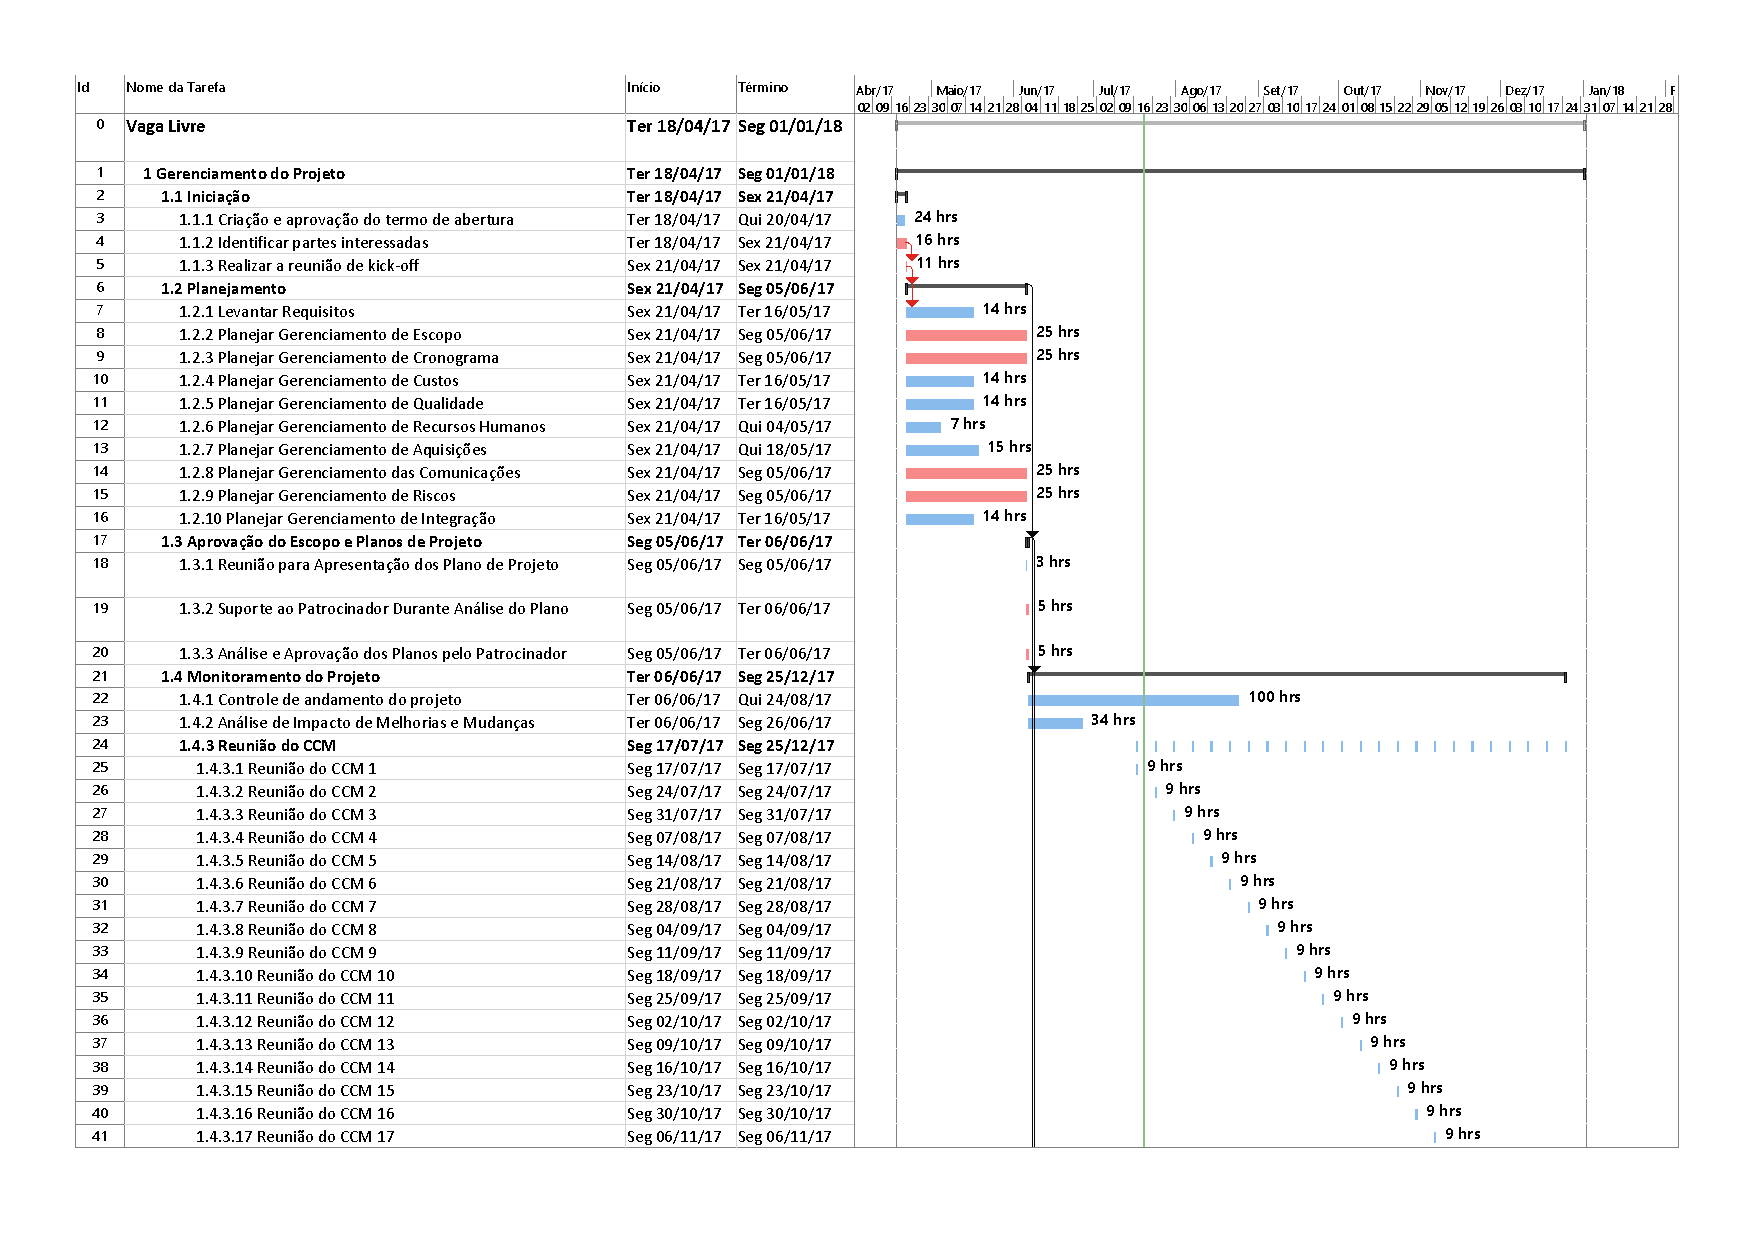
\includepdf[landscape=true,turn=false,pages=1,pagecommand={\chapter{Gráfico Gannt}\label{ch:gannt-chart}},linktodoc=true]{include/gannt.pdf}
\includepdf[landscape=true,turn=false,pages=2-,pagecommand={}]{include/gannt.pdf}

	%\chapter{Listas de verificação de qualidade}

	\begin{landscape}

	\chapter{Métricas de qualidade}
	\label{quality-metrics}

	\begin{longtable}{ p{0.08\textwidth} p{0.08\textwidth}  p{0.08\textwidth}  p{0.08\textwidth}  p{0.08\textwidth} p{0.08\textwidth} p{0.08\textwidth} p{0.08\textwidth}  p{0.08\textwidth}  p{0.08\textwidth}  p{0.08\textwidth} p{0.08\textwidth} p{0.08\textwidth} }
		\toprule
		\rot{\textbf{\parbox{4cm}{Nome da\\ Métrica}}} & \rot{\textbf{\parbox{4cm}{Descrição}}} & \rot{\textbf{\parbox{4cm}{Forma de\\ Cálculo}}} & \rot{\textbf{\parbox{4cm}{Unidade}}} & \rot{\textbf{\parbox{4cm}{Meta}}} & \rot{\textbf{\parbox{4cm}{Periodicidade\\ da Coleta}}} & \rot{\textbf{\parbox{4cm}{Responsável\\ pela Coleta}}} & \rot{\textbf{\parbox{4cm}{Local de\\ Coleta}}} & \rot{\textbf{\parbox{4cm}{Armazenamento\\ do Resultado}}} & \rot{\textbf{\parbox{4cm}{Procedimento\\ para Análise}}} & \rot{\textbf{\parbox{4cm}{Responsável\\ pela Análise}}} & \rot{\textbf{\parbox{4cm}{Frequência de\\ Divulgação}}} & \rot{\textbf{\parbox{4cm}{Destinatário\\ da Informação}}} \\
		\midrule
         & & & & & & & & & & & & \\
        \bottomrule
		\centering
		\caption{Métricas de qualidade.}
	\end{longtable}

\end{landscape}

\end{apendicesenv}
% ---

% ----------------------------------------------------------
% Attachments
% ----------------------------------------------------------

% ---
% Attachments begin
% ---
\begin{anexosenv}

	% Print page indicating the attachments session begin
	\partanexos

	% ---
	\chapter{Diferença entre Anexo e Apêndice}
	% ---
	Segundo a NBR 14724 de dezembro de 2005, a diferença primordial entre Anexo e Apêndice é que o Anexo é um texto ou documento não elaborado pelo autor do Trabalho Científico (TC) (monografia, tese, etc.) e o Apêndice é um texto ou documento elaborado pelo autor do TC, ou seja, se foi necessário você criar uma entrevista, um relatório, ou qualquer documento com o escopo de complementar sua argumentação, deve-se utilizar o termo Apêndice e não Anexo.

	Exemplos:

	ANEXO A – Documento ou texto não elaborado pelo autor

	APÊNDICE A – Documento ou texto elaborado pelo autor

\end{anexosenv}

%---------------------------------------------------------------------
% INDICE REMISSIVO
%---------------------------------------------------------------------
\phantompart
\printindex
%---------------------------------------------------------------------

\end{document}